\documentclass[11 pt,t]{beamer}
\usetheme[
	bullet=circle,		% Other option: square
	bigpagenumber,		% circled page number on lower right
	topline=true,		% colored bar at the top of the frame 
	]{Zurich}


%-----------------------------------------------------------------------------
% DOCUMENT PROPERTIES
\usepackage[export]{adjustbox}
\usepackage{amsmath}
\usepackage{xfrac}
\usepackage{amssymb}
\usepackage{blkarray}
\newcommand{\fw}{0.75\linewidth} % large figure width
\newcommand{\gw}{0.4\linewidth} % graph width
\newcommand{\tw}{0.6\linewidth} % time series width

%tikz -----------------------------

\usepackage{tikz,pgfplots}
\usetikzlibrary{arrows,calc}

\usepackage{etoolbox}

\newenvironment{customlegend}[1][]{%
    \begingroup
    % inits/clears the lists (which might be populated from previous
    % axes):
    \csname pgfplots@init@cleared@structures\endcsname
    \pgfplotsset{#1}%
}{%
    % draws the legend:
    \csname pgfplots@createlegend\endcsname
    \endgroup
}%

% makes \addlegendimage available (typically only available within an
% axis environment):
\def\addlegendimage{\csname pgfplots@addlegendimage\endcsname}

%%--------------------------------

% definition to insert numbers
\pgfkeys{/pgfplots/number in legend/.style={%
        /pgfplots/legend image code/.code={%
            \node at (0.295,-0.0225){#1};
        },%
    },
}

% --------- New commands -----


\newcommand{\myparagraph}[1]{\paragraph{#1}\mbox{}\\}
\newcommand{\PP}{\textit{\tiny P}}
\newcommand{\CC}{\textit{\tiny C}}
\newcommand{\R}{\textit{\tiny R}}
\newcommand{\CR}{\textit{\tiny CR}}
\newcommand{\PC}{\textit{\tiny PC}}
\newcommand{\PR}{\textit{\tiny PR}}
\newcommand{\CP}{\textit{\tiny CP}}
\newcommand{\RC}{\textit{\tiny RC}}
\newcommand{\RP}{\textit{\tiny RP}}

% -------------------------------------

\author{Carlos Andres Marcelo Serv\'an}
\title[Tesis para optar el t\'itulo de Bi\'ologo]{Influencia de la raz\'on de masas depredador-presa sobre la longitud
  de las cadenas tr\'oficas}
\institute{\color{tangocolordarkskyblue}
  Universidad Nacional Mayor de San Marcos, Ciencias Biol\'ogicas\\
  $\bigstar$ \texttt{cmarceloservan@uchicago.edu}
}
\date{15 de Agosto 2017}
%-----------------------------------------------------------------------------
\begin{document}
% ----------------------------------------------------------------------------
\frame{

\titlepage

}
% ----------------------------------------------------------------------------
\begin{frame}
  \frametitle{Cad\'enas tr\'oficas}
  
  \centering
  
  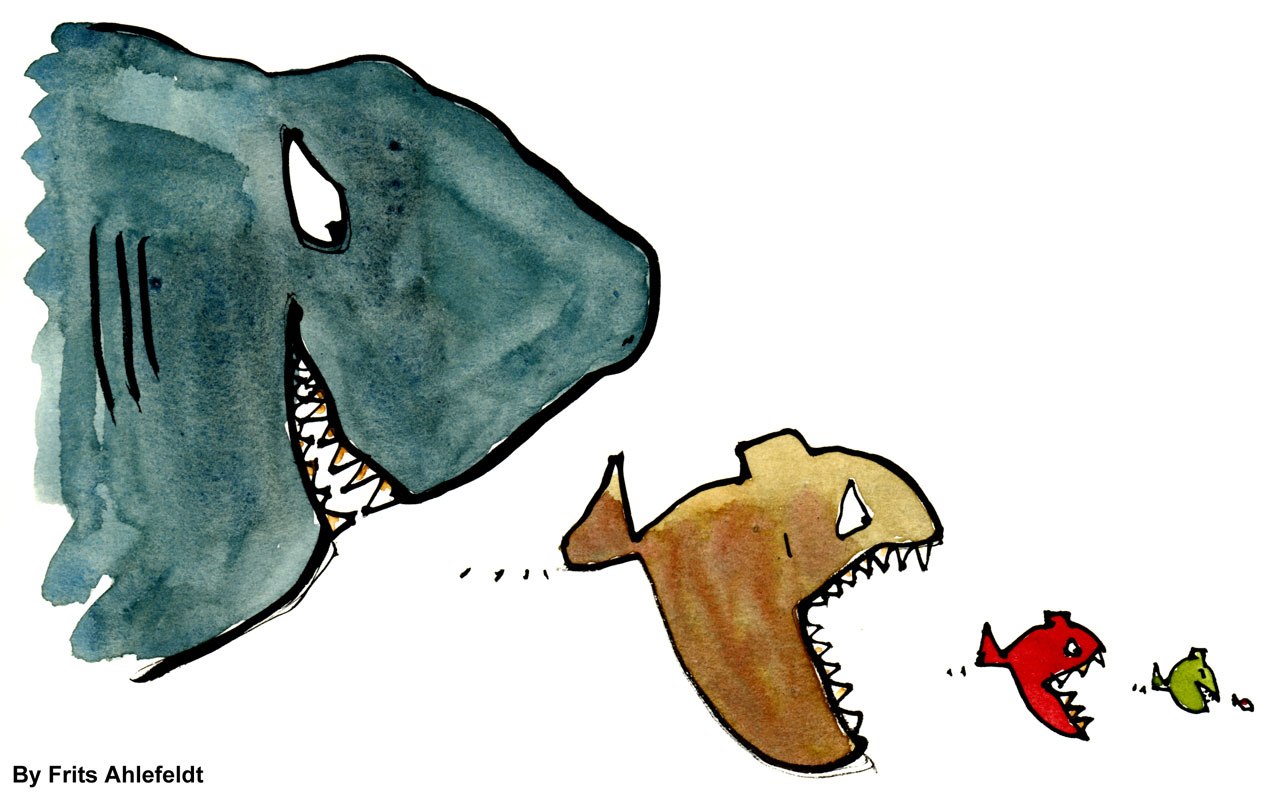
\includegraphics[width = 0.7\linewidth]{Pics/fishes.jpeg}

\end{frame}
% ----------------------------------------------------------------------------
\begin{frame}
  \frametitle{Redes tr\'oficas}
  
  \centering
  
  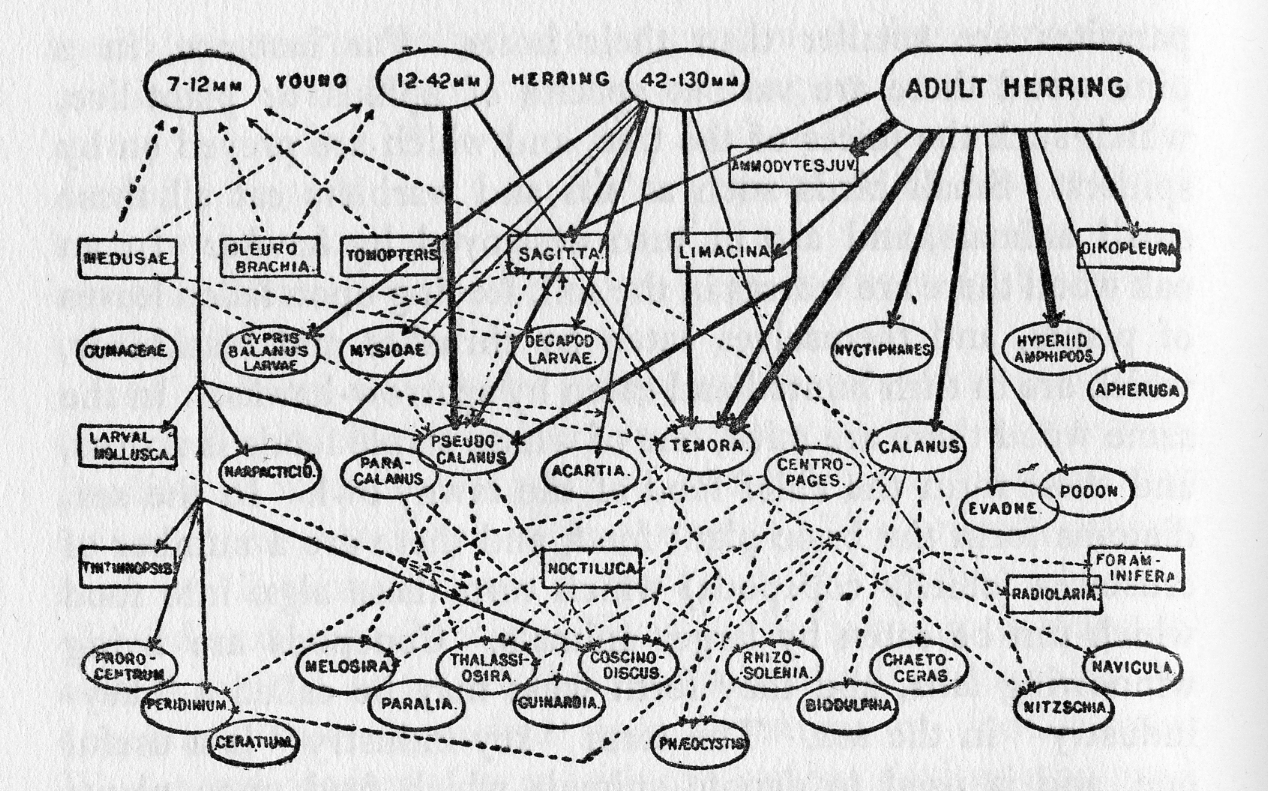
\includegraphics[width = 0.8\linewidth]{Pics/fw.jpg}
  \tiny Elton, Animal Ecolofy 1926.
\end{frame}

% ----------------------------------------------------------------------------

\begin{frame}
  \frametitle{Niveles tr\'oficos}
  \centering
  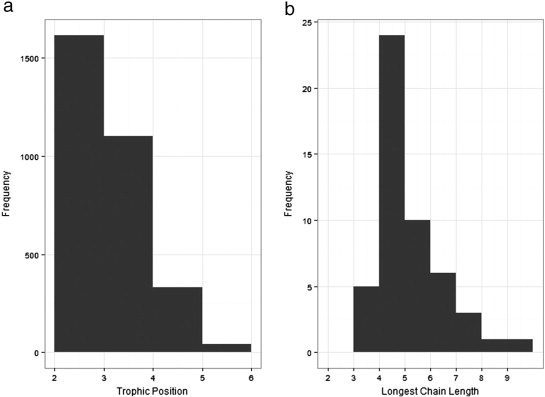
\includegraphics[width = 0.7\linewidth]{Pics/mtp.jpg} \\
  \tiny Borrelli y Ginzburg, Food Webs 2014
\end{frame}
% ---------------------------------------------------------------------------
\begin{frame}
  \frametitle{¿Qu\'e limita la longitud de las cadenas tr\'oficas?}  \centering
  \centering
  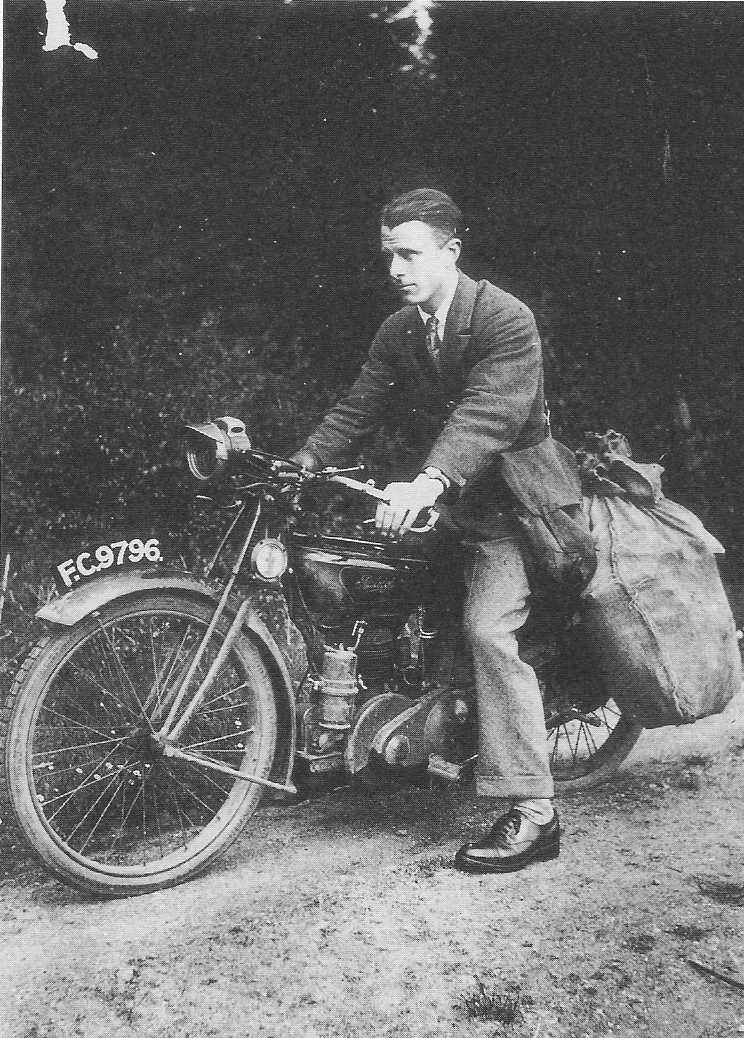
\includegraphics[width = 0.3\linewidth]{Pics/Elton.jpg}
        
  \begin{equation*}
    TP_j = \sum_{i \in G} (1+TP_i) p_i 
  \end{equation*}
   
\end{frame}
% ----------------------------------------------------------------------------
\begin{frame}
  \frametitle{Muchas cosas...}
  
  \begin{itemize}
    \item Estabilidad
    \item Productividad del ambiente
    \item Tama\~no del ecosistema
    \item R\'egimen de disturbancias
    \item Historia comunitaria
    \item Tipos de interacciones depredador-presa
  \end{itemize}

\Large \begin{quote}``The debate now shifts away from a search for a single explanation for variation in food-chain length to a search for when and where a suite of interacting constraints operates to determine variation in food-chain length''\footnote{Post .Trends in Ecology and Evolution 2002} \end{quote}
\end{frame}

% ---------------------------------------------------------------------------
\begin{frame}
  \frametitle{Ley de Kleiber} 
  \centering
  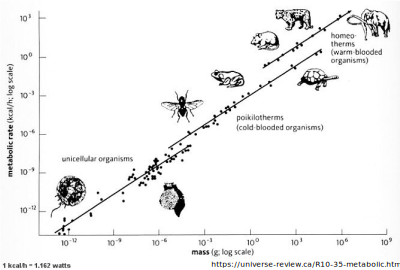
\includegraphics[width = 0.7\linewidth]{Pics/mscaling.pdf}
  \begin{equation} I \propto m^{\beta} \end{equation}
  Una derivaci\'on de esta relaci\'on con $\beta = 3/4$ se da en West \textit{et al.} Nature 1997
\end{frame}
% ---------------------------------------------------------------------------
\begin{frame}
  \frametitle{Teor\'ia Metab\'olica de la Ecolog\'ia\footnote{Brown. Ecology 2005}}
  \begin{quote}{Brown \textit{et al.} 2012}
    ``Metabolism is defined as the transformation of energy and materials within and organism''
  \end{quote}
  
  \begin{itemize}
  \item \begin{equation} B \propto m^{\beta - 1}e^{-E/kT} \end{equation}
  \item \begin{equation} r \propto m^{\beta - 1}e^{-E/kT} \end{equation}
  \item \begin{equation} q \propto m^{\beta - 1}e^{-E/kT} \end{equation}
  \item \begin{equation} K \propto m^{1 - \beta}e^{E/kT} \end{equation}
  \end{itemize}
  
\end{frame}
% ---------------------------------------------------------------------------
\begin{frame}
  \frametitle{Masa corporal e interacciones depredador-presa}
  \centering
      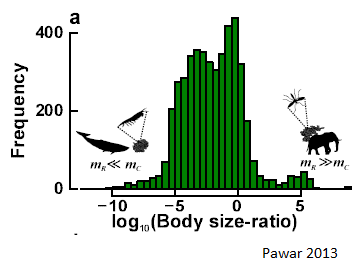
\includegraphics[width = 0.7\linewidth]{Pics/bz.png}      
\end{frame}
% ----------------------------------------------------------------------------
\begin{frame}
  \frametitle{Dimensionalidad de las interacciones}
  \centering
  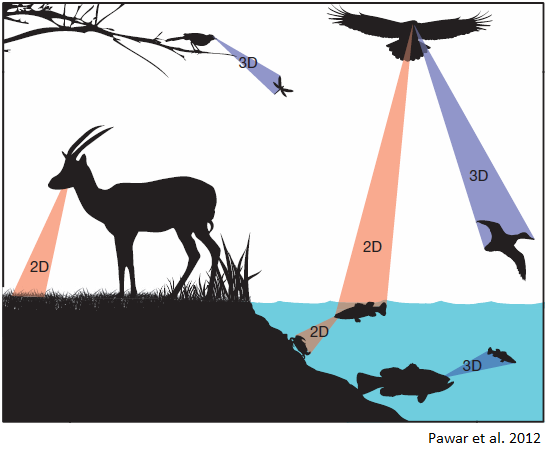
\includegraphics[width = 0.7\linewidth]{Pics/dimensionality.png}      
\end{frame}
% ----------------------------------------------------------------------------
\begin{frame}
  \frametitle{Estrategias de forrajeo}
  \centering
  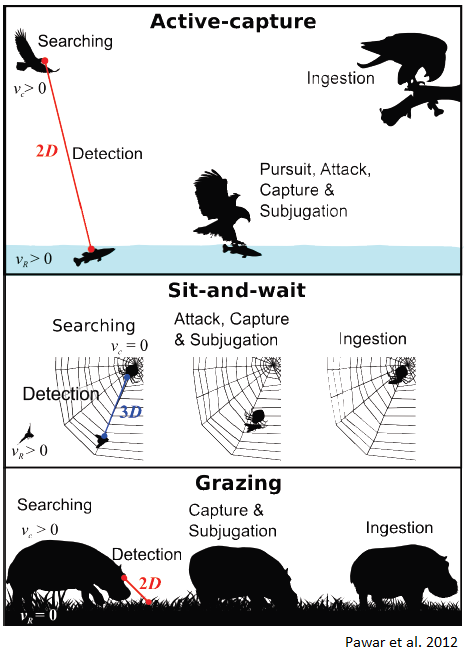
\includegraphics[width = 0.5\linewidth]{Pics/capture.png}
\end{frame}
% ---------------------------------------------------------------------------
\begin{frame}
  \frametitle{Derivaci\'on de la tasa de ataque $\alpha$\footnote{Pawar \textit{et al.} 2012; Kiltie, 2000; McGill y Miltebach 2006}}
  \begin{equation}
    \begin{aligned}
      m_j\alpha & =  S_A*\aleph \\
      S_A &=  A_D * v_r \\
      A_D &=  \begin{cases} 2d & \text{si } D_i = 2 \\ \pi d^2 & \text{si } D_i = 3 \end{cases}\\
      v_r &= \sqrt{v_i^2 +v_j^2}\\
      \aleph &= \Pi(k_{ij}) \\
    \end{aligned}
  \end{equation}
  \begin{columns}
    \begin{column}{0.4\textwidth}
      \begin{flalign*}
        \Pi(k_{ij}) &=\frac{a}{1+k_{ij}^\phi}
        \end{flalign*}
  \end{column}
  \begin{column}{0.6\textwidth}
    \begin{center}
      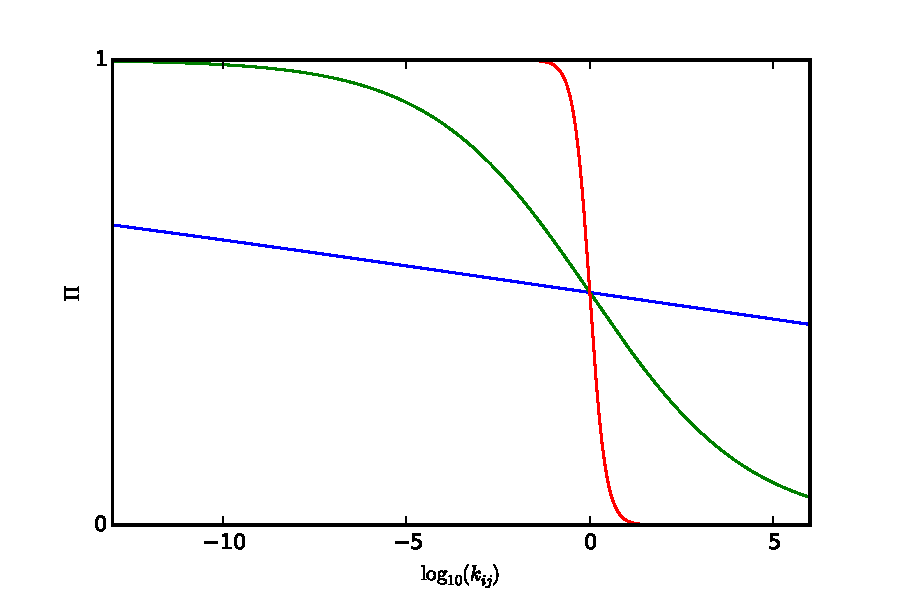
\includegraphics[width = 0.6\textwidth]{../manuscript/Plots/CaptureEfficiency.pdf}
      \end{center}
      \end{column}
      
    \end{columns}
    
\end{frame}

% ---------------------------------------------------------------------------
\begin{frame}
  \frametitle{Derivaci\'on de la tasa de ataque $\alpha$\footnote{Pawar \textit{et al.} 2012; Kiltie, 2000; McGill y Miltebach 2006}}
  Tomando
  \begin{equation}
    \begin{aligned}
      d &\propto (m_im_j)^{p_d} \\
      v &\propto m^{\beta - \beta_F}
    \end{aligned}
  \end{equation}

  Tenemos:
  \begin{equation}
    \alpha \propto m_j^{p_v+2p_d(D-1) - 1}f(k_{ij})
  \end{equation}

  Dependiendo de la estrategia de forrajeo $f$ toma las siguientes formas:
  \begin{equation}\label{eq:fkr}
    f(k_{ij}) = 
    \begin{cases}
      \sqrt{1+k_{ij}^{2p_v}}k_{ij}^{(D_j-1)p_d} \Pi(k_{ij}) & Fm = Ac\\
      k_{ij}^{p_v+(D_j-1)p_d}\Pi(k_{ij}) & Fm = Sw\\
      k_{ij}^{(D_j-1)p_d}\Pi(k_{ij}) & Fm = Gr\\
    \end{cases}
  \end{equation}

  
\end{frame}

% ---------------------------------------------------
\begin{frame}
  \frametitle{$f$}
  \centering
  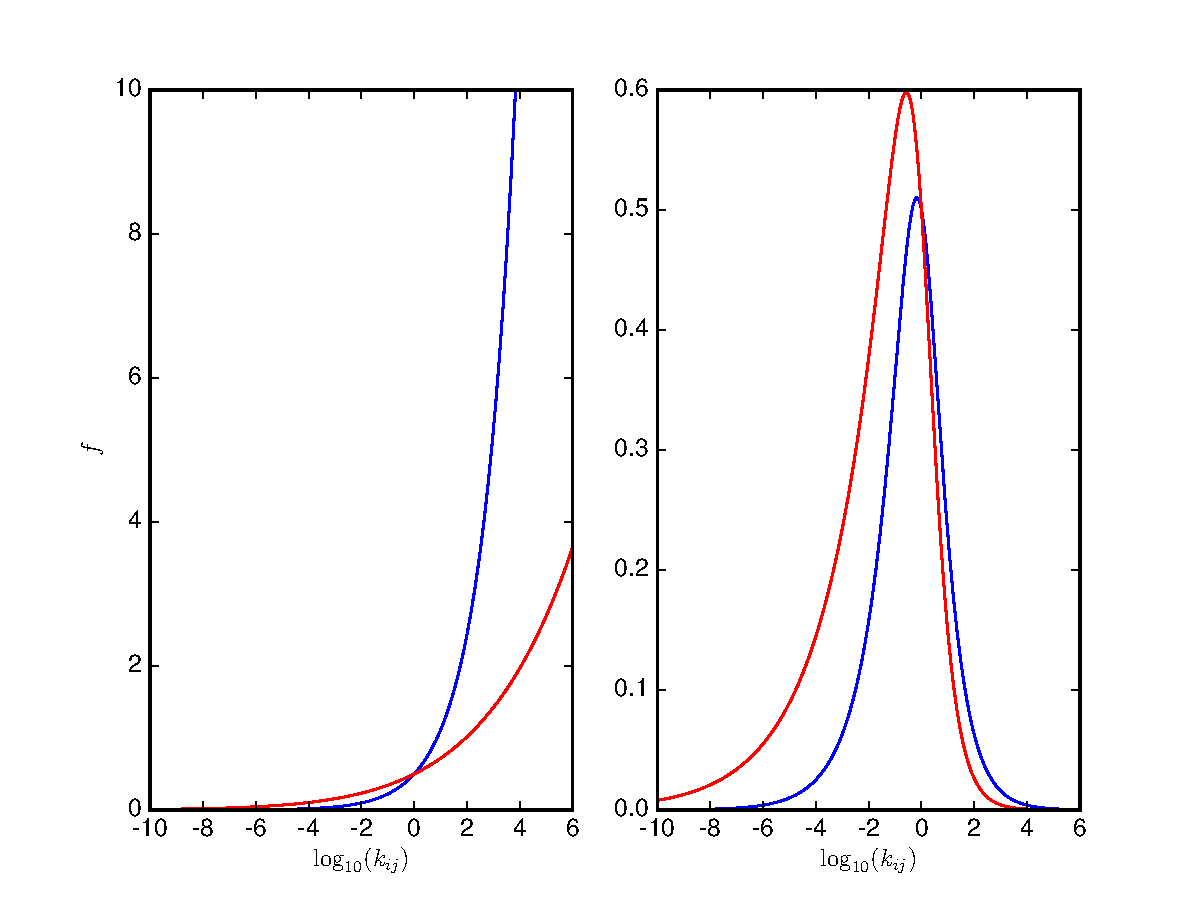
\includegraphics[width=0.9\textwidth]{../manuscript/Plots/f1Grazing.pdf}
\end{frame}
% ---------------------------------------------------
\begin{frame}
  \frametitle{Modelaci\'on matem\'atica}
  \Large
  \begin{equation}
    \frac{dx}{dt} = xF(x)
  \end{equation}
  \Large \textit{Lotka Volterra}
  \begin{equation}
    \frac{dx_i}{dt} = x_i (r_i + \sum_j \alpha_{ij}x_j)
  \end{equation}
\end{frame}
% ----------------------------------------------------------------------------
\begin{frame}
  \frametitle{M\'odulo de depredaci\'on Intragremial \footnote{Polis \textit{et al.} 1989}}
  \centering
  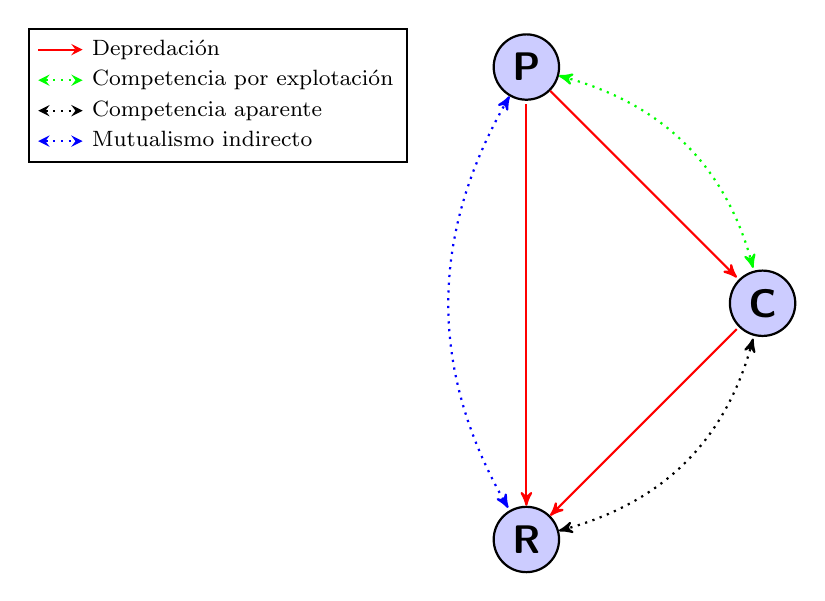
\begin{tikzpicture}[<->,>=stealth',shorten >=1pt,auto,
  thick,main node/.style={circle,fill=blue!20,draw,font=\sffamily\Large\bfseries}]


\node[main node] (R) at (0,-3){R};
\node[main node] (C) at (3,0) {C};
\node[main node] (P) at (0,3) {P};

 \path[every node/.style={font=\sffamily\small}]

(R) edge [<-,red] (C)
(R) edge [<-,red] (P)
(P) edge [->,red] (C)
(P) edge [bend right , dotted, blue] (R) 
(P) edge [bend left , dotted, green]  (C)
(R) edge [bend right ,dotted , black] (C);



\begin{customlegend}[legend cell align=left,
legend entries={ % <= in the following there are the entries
Depredaci\'on,
Competencia por explotaci\'on,
Competencia aparente, 
Mutualismo indirecto
},
legend style={at={(-1.5,3.5)},font=\footnotesize}] % <= to define position and font legend
% the following are the "images" and numbers in the legend
    \addlegendimage{-stealth,red}
    \addlegendimage{stealth-stealth,dotted,green}
    \addlegendimage{stealth-stealth,dotted,black}
    \addlegendimage{stealth-stealth,dotted,blue}
    
\end{customlegend}

\end{tikzpicture}

\end{frame}
% ---------------------------------------------------------------------------

\begin{frame}
  \frametitle{Caminos de Ensamblaje}
  \centering
  \resizebox{0.8\textwidth}{!}{
    
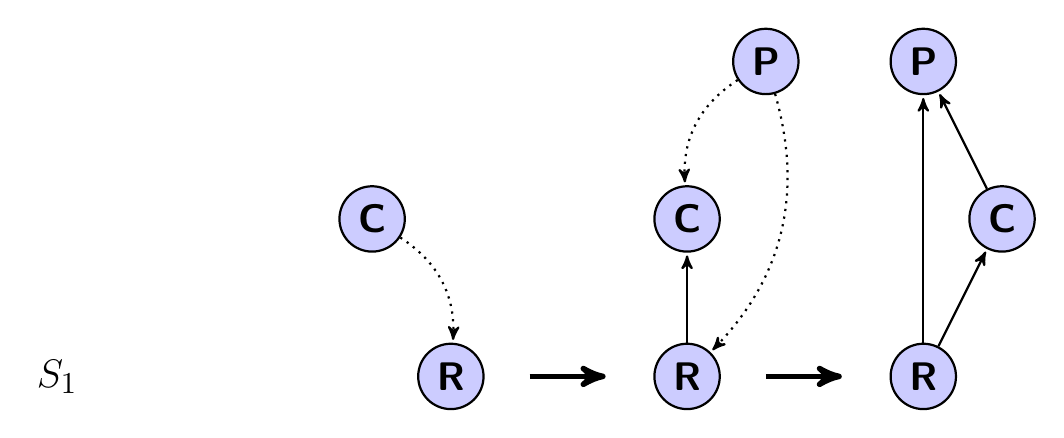
\begin{tikzpicture}[->,>=stealth',shorten >=1pt,auto,
  thick,main node/.style={circle,fill=blue!20,draw,font=\sffamily\Large\bfseries}]

\node[main node](R1) at (1,0) { R};
\node[main node](C1) at (0,2) {C};
\node[main node](C2) at  (4,2){C};
\node[main node](R2) at ($(R1) + (3,0)$) {R};
\node[main node](P1) at (5,4){P};
\node[main node](R3) at ($(R2) + (3,0)$){R};
\node[main node](C3) at ($(R3) + (1,2)$){C};
\node[main node](P3) at ($(R3) + (0,4)$){P};
\node[font = \fontsize{15}{15}\selectfont](A1) at (-4,0) {$S_1$};

\path
(C1) edge[bend left,dotted] (R1)
($(R1)+(1.0,0)$) edge[line width = 2]  ($(R1)+ (2,0)$)
(R2) edge (C2)
(P1) edge[bend right,dotted] (C2)
(P1) edge[bend left,dotted] (R2)
($(R2) + (1.0,0)$) edge[line width  = 2] ($(R2) + (2,0)$)
(R3) edge (C3)
(R3) edge (P3)
(C3) edge (P3);
\end{tikzpicture}
}
\resizebox{0.8\textwidth}{!}{

  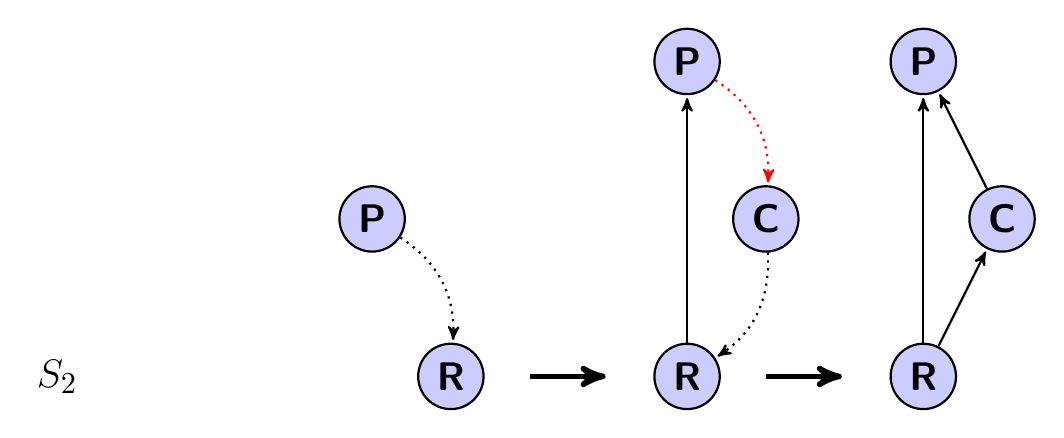
\begin{tikzpicture}[->,>=stealth',shorten >=1pt,auto,
  thick,main node/.style={circle,fill=blue!20,draw,font=\sffamily\Large\bfseries}]

\node[main node](R1) at (1,0) { R};
\node[main node](P1) at (0,2) {P};
\node[main node](P2) at  (4,4){P};
\node[main node](R2) at ($(R1) + (3,0)$) {R};
\node[main node](C1) at (5,2){C};
\node[main node](R3) at ($(R2) + (3,0)$){R};
\node[main node](C3) at ($(R3) + (1,2)$){C};
\node[main node](P3) at ($(R3) + (0,4)$){P};
\node[font = \fontsize{15}{15}\selectfont](A1) at (-4,0) {$S_2$};

\path
(P1) edge[bend left,dotted] (R1)
($(R1)+(1.0,0)$) edge[line width = 2]  ($(R1)+ (2,0)$)
(R2) edge (P2)
(C1) edge[bend left,dotted] (R2)
(P2) edge[bend left,dotted,red] (C1)
($(R2) + (1.0,0)$) edge[line width  = 2] ($(R2) + (2,0)$)
(R3) edge (C3)
(R3) edge (P3)
(C3) edge (P3);

\end{tikzpicture}
}
\end{frame}
% ---------------------------------------------------------------------------

\begin{frame}
  \begin{tikzpicture}[<->,>=stealth',shorten >=0.1pt,auto,
  thick,main node/.style={circle,fill=blue!20,draw,font=\sffamily\Large\bfseries}]


\node (fig1) at (-3,-5)
       {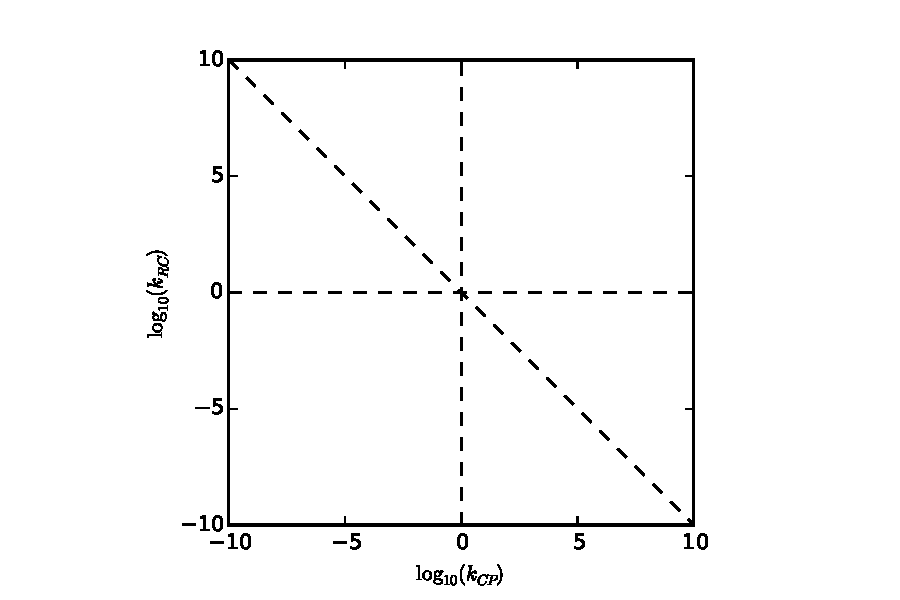
\includegraphics[scale=0.8]{C:/Users/Carlos/Documents/Tesis-IGP/code/Theory/ZonesSR.pdf}};

\node[circle,fill= blue!20,draw, minimum size=0.6cm,inner sep= 0] (R) at (-5.5,-4.5){R};
\node[circle,fill=blue!20,draw,minimum size=0.3cm, inner sep = 0] (C) at (-4.5,-3.8) {C};
\node[circle,fill=blue!20,draw,minimum size=1.cm,inner sep = 0](P) at (-5.5,-3.) {P};

 \path[every node/.style={font=\sffamily\small}]

(R) edge [<-,red] (C)
(R) edge [<-,red] (P)
(P) edge [->,red] (C);


\node[circle,fill= blue!20,draw, minimum size=0.3cm,inner sep= 0] (R) at (-4.5,-7.8){R};
\node[circle,fill=blue!20,draw,minimum size=0.6cm, inner sep = 0] (C) at (-3.5,-6.7) {C};
\node[circle,fill=blue!20,draw,minimum size=1.cm,inner sep = 0](P) at (-4.5,-5.6) {P};

 \path[every node/.style={font=\sffamily\small}]

(R) edge [<-,red] (C)
(R) edge [<-,red] (P)
(P) edge [->,red] (C);


\node[circle,fill= blue!20,draw, minimum size=1.cm,inner sep= 0] (R) at (-3.4,-3.6){R};
\node[circle,fill=blue!20,draw,minimum size=0.3cm, inner sep = 0] (C) at (-4.3,-2.6) {C};
\node[circle,fill=blue!20,draw,minimum size=0.6cm,inner sep = 0](P) at (-3.4,-2.1) {P};

 \path[every node/.style={font=\sffamily\small}]

(R) edge [<-,red] (C)
(R) edge [<-,red] (P)
(P) edge [->,red] (C);



\node[circle,fill= blue!20,draw, minimum size=1.cm,inner sep= 0] (R) at (-1.5,-4.1){R};
\node[circle,fill=blue!20,draw,minimum size=0.6cm, inner sep = 0] (C) at (-0.3,-3) {C};
\node[circle,fill=blue!20,draw,minimum size=0.3cm,inner sep = 0](P) at (-1.5,-2.1) {P};

 \path[every node/.style={font=\sffamily\small}]

(R) edge [<-,red] (C)
(R) edge [<-,red] (P)
(P) edge [->,red] (C);


\node[circle,fill= blue!20,draw, minimum size=0.6cm,inner sep= 0] (R) at (-0.1,-7){R};
\node[circle,fill=blue!20,draw,minimum size=1.0cm, inner sep = 0] (C) at (-1,-5.9) {C};
\node[circle,fill=blue!20,draw,minimum size=0.3cm,inner sep = 0](P) at (-0.1,-5.2) {P};

 \path[every node/.style={font=\sffamily\small}]

(R) edge [<-,red] (C)
(R) edge [<-,red] (P)
(P) edge [->,red] (C);


\node[circle,fill= blue!20,draw, minimum size=0.3cm,inner sep= 0] (R) at (-2.55,-7.8){R};
\node[circle,fill=blue!20,draw,minimum size=1.cm, inner sep = 0] (C) at (-1.8,-6.7) {C};
\node[circle,fill=blue!20,draw,minimum size=0.6cm,inner sep = 0](P) at (-2.55,-5.7) {P};

 \path[every node/.style={font=\sffamily\small}]

(R) edge [<-,red] (C)
(R) edge [<-,red] (P)
(P) edge [->,red] (C);


   
\end{tikzpicture}
  
\end{frame}
% ---------------------------------------------------------------------------
\begin{frame}
  \frametitle{Parameterizaci\'on bioenerg\'etica}
  \centering
  \begin{equation}
    \begin{aligned} 
      \frac{dR}{dt} &= R\left[ r(1-\frac{R}{K})- \alpha_1 C -\alpha_2 P \right] \\
      \frac{dC}{dt} &= C \left[ \epsilon_1 \alpha_1 R - \alpha_3  P - q_1 \right] \\
      \frac{dP}{dt} &= P \left[ \epsilon_2 \alpha_2 R + \epsilon_3 \alpha_3 C - q_2 \right]
    \end{aligned}
  \end{equation}

  \begin{equation}\label{eq:params3}
\begin{aligned}
&r = r_0m_{\R}^{\beta - 1} \\
&q_1=q_{0,1}m_{\CC}^{\beta - 1} \\
&q_2= q_{0,2}m_{\PP}^{\beta -1}\\
&K= \kappa_{0}m_{\R}^{1-\beta}\\
&m_{\CC} \alpha_1= \alpha_{0,1}m_{\CC}^{p_v+2p_d(D - 1)}f_1(k_{\RC})\\
\end{aligned}
\end{equation}
\end{frame}
% ---------------------------------------------------------------------------
\begin{frame}
  \frametitle{An\'alisis de Invasibilidad}
  \Large Supuestos:
  \begin{itemize}
    \item \emph{El sistema receptor se ha encontrado aislado por suficiente tiempo como para alcanzar un estado asimpt\'otico y dicho estado es un punto de equilibrio}
    \item \emph{La invasi\'on se considera exitosa si es que existe un crecimiento por parte del invasor en los instantes posteriores a la invasi\'on}
    \end{itemize}
\end{frame}
% ---------------------------------------------------------------------------
\begin{frame}
  \frametitle{\resizebox{0.3in}{0.3in}{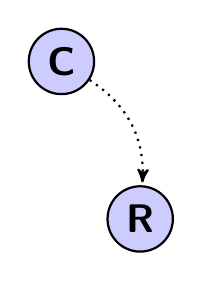
\begin{tikzpicture}[->,>=stealth',shorten >=1pt,auto,
  thick,main node/.style={circle,fill=blue!20,draw,font=\sffamily\Large\bfseries}]

  \node[main node](R1) at (1,0) { R};
  \node[main node](C1) at (0,2) {C};

  \path
  (C1) edge[bend left,dotted] (R1);

\end{tikzpicture}

} $\;\;$ Invasibilidad $C \to R$}
  \begin{equation}
    \frac{dC}{dt} > 0 \iff  \mu_1 := (m_P^w > \zeta_1(k_{\CP},k_{\RC}) = k^{-w}_{\CP} \frac{q_{0,1}}{\chi_1})
  \end{equation}
  Donde:
  \begin{equation}
    \begin{aligned}
      h_R &= p_v + 2(D_R - 1)p_d \\
      w &= h_R + 1 - 2 \beta \\
      \chi_1 &= \varepsilon_1 \kappa_0\alpha_{0,1} g(k_{\RC}) \\
      g(k_{\RC}) &= f_1(k_{\RC})k_{\RC}^{1-\beta}\\
    \end{aligned}
  \end{equation}
\end{frame}
% ---------------------------------------------------------------------------
\begin{frame}
  \frametitle{\resizebox{0.3in}{0.3in}{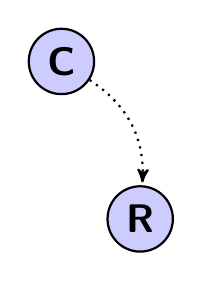
\begin{tikzpicture}[->,>=stealth',shorten >=1pt,auto,
  thick,main node/.style={circle,fill=blue!20,draw,font=\sffamily\Large\bfseries}]

  \node[main node](R1) at (1,0) { R};
  \node[main node](C1) at (0,2) {C};

  \path
  (C1) edge[bend left,dotted] (R1);

\end{tikzpicture}

} $\;\;$ $C \to R$}
  \begin{equation}
\mathbf{Z(I_{\CC \to \R})} := \{ (k_{\RC},k_{\CP},m_P) \in \mathbb{R}^3_+ / m_p^{h_R + 1 - 2\beta} > \zeta_1(k_{\RC},k_{\CP}) \}
\end{equation}

\centering
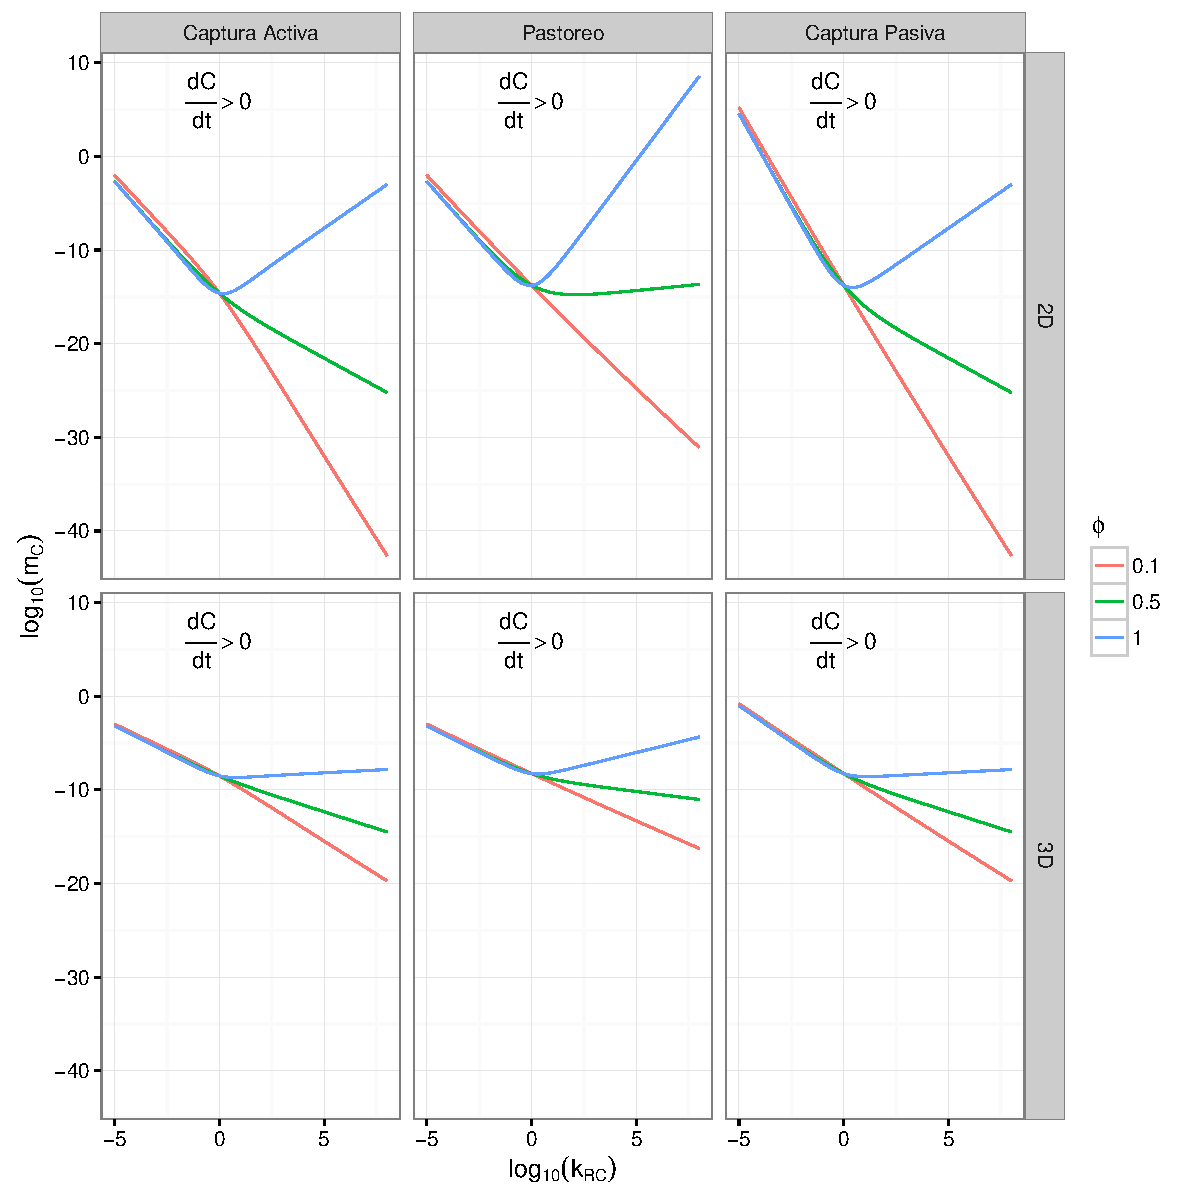
\includegraphics[width = 0.6\textwidth]{../manuscript/Plots/R-CInv.pdf}

\end{frame}

% ---------------------------------------------------------------------------
\begin{frame}
  \frametitle{Invasibilidad $P \to R$}
  \begin{equation}
    \frac{dP}{dt} >0 \iff \mu_2 := ( m_P^{h_R + 1 - 2\beta} > \zeta_2(k_{\RC},k_{\CP}) = \frac{q_{0,2}}{\chi_2} )
  \end{equation}

  \begin{equation}
    \begin{aligned}
      \chi_2 &= \varepsilon_2 \kappa_0\alpha_{0,2} f_2(k_{\RP})k_{\RP}^{1-\beta} \\
    \end{aligned}
  \end{equation}

  \begin{equation}
    \mathbf{Z(I_{\PP \to \R})} := \{ (k_{\RC},k_{\CP},m_P) \in \mathbb{R}^3_+ / m_p^{h_R + 1 - 2\beta} > \zeta_2(k_{\RC},k_{\CP}) \}
  \end{equation}

\end{frame}
% ----------------------------------------------------------------------------
\begin{frame}
  \frametitle{Invasibilidad $P \to C-R$}
  \begin{columns}
    \begin{column}{0.7\textwidth}
    \begin{equation*}
      \begin{aligned}
      \mu_3 &:= (\gamma_1 = \chi_3 + \chi_4 - q_{0,2} >0 \ \land \\ &m_P^{h + 1 - 2\beta} > \zeta_3(k_{\RC},k_{\CP}) = \frac{\chi_4}{\chi_3 + \chi_4 - q_{0,2}}\zeta_1)
    \end{aligned}
  \end{equation*}
  \end{column}
  
  \begin{column}{0.3\textwidth}
    \begin{center}
      \resizebox{0.3\textwidth}{!}{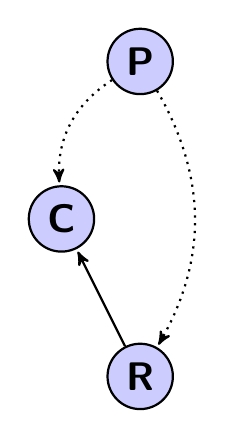
\begin{tikzpicture}[->,>=stealth',shorten >=1pt,auto,
  thick,main node/.style={circle,fill=blue!20,draw,font=\sffamily\Large\bfseries}]

\node[main node](R1) at (1,0) { R};
\node[main node](C1) at (0,2) {C};
\node[main node](P1) at (1,4){P};

\path
(R1) edge (C1)
(P1) edge[bend right,dotted] (C1)
(P1) edge[bend left,dotted] (R1);
\end{tikzpicture}

}
      \end{center}
  \end{column}
  \end{columns}
Donde:
\begin{equation}\label{eq:3rdCond}
  \begin{aligned}
    \chi_3 &= \chi_2 \zeta_1 \\
    \chi_4 &= \frac{\varepsilon_3 \alpha_{0,3}r_0 f_3(k_{\CP})k_{\CP}^{\beta - h}}{\alpha_{0,1}f_1(k_{\RC})k_{\RC}^{1-\beta}}
  \end{aligned}
\end{equation}

\begin{equation}
    \mathbf{Z(I_{\PP \to \CC-\R})} := \{ (k_{\RC},k_{\CP},m_P) \in \mathbb{R}^3_+ / \mu_1 \land \mu_3 \}
  \end{equation}


\end{frame}
% ---------------------------------------------------------------------------
\begin{frame}
  \frametitle{$P \to C-R$}
  \tiny
  \begin{equation}
    \varepsilon_2 \alpha_2 R_2^* + \varepsilon_3 \alpha_3 \frac{r}{\alpha_1} > q_2
  \end{equation}
  \centering
  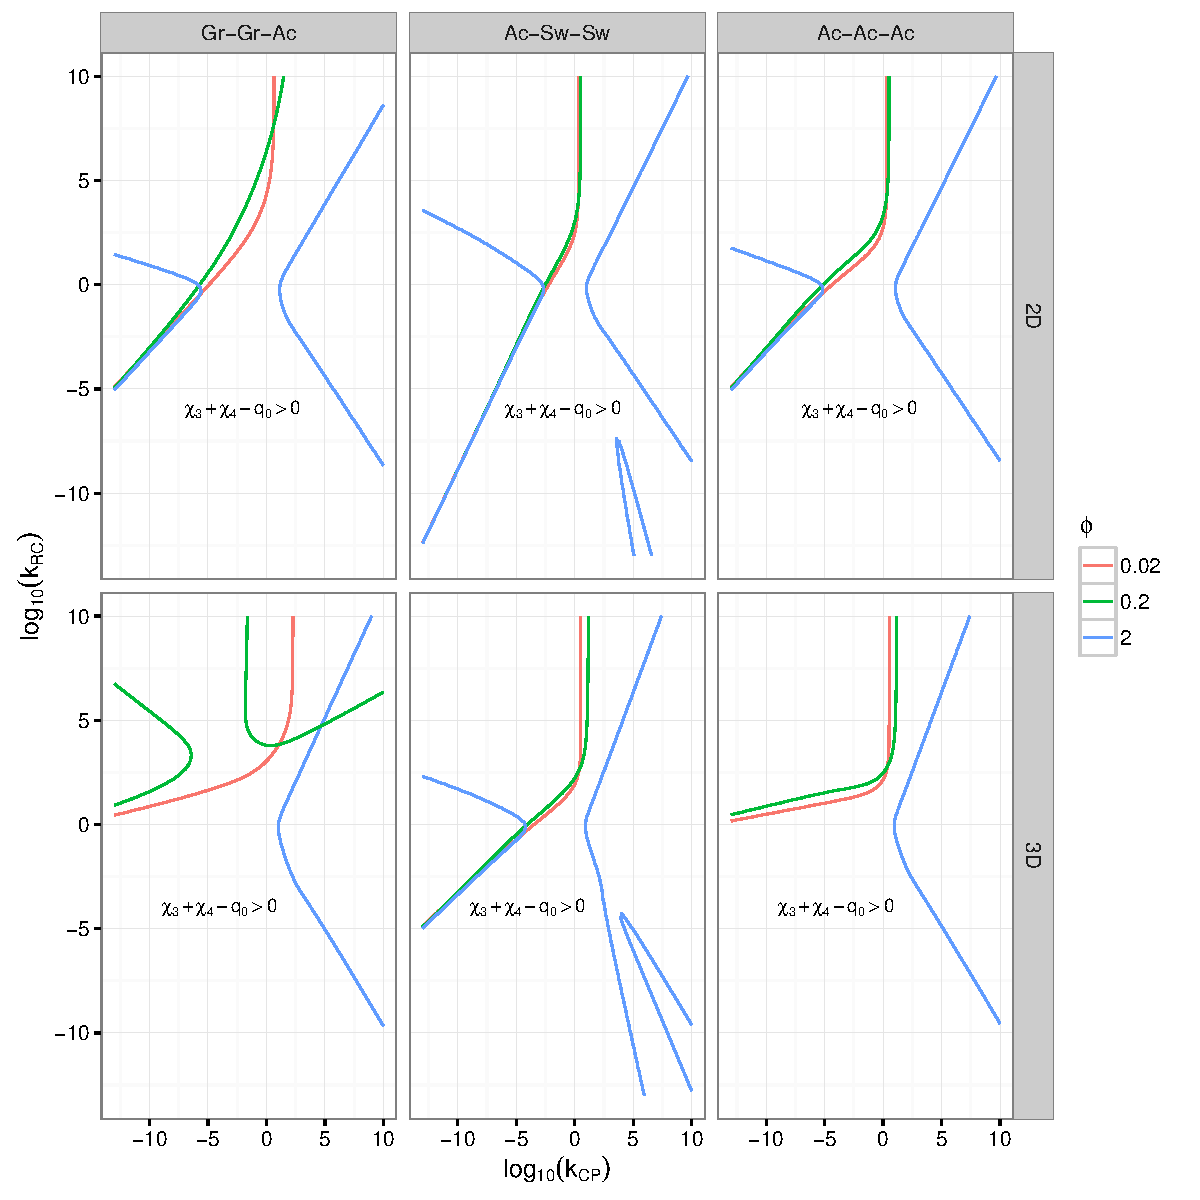
\includegraphics[width = 0.65\textwidth]{../manuscript/Plots/NecPCR.pdf}
\end{frame}

% --------------------------------------------------------------------------
\begin{frame}
  \frametitle{$P \to C-R$}
  \centering
  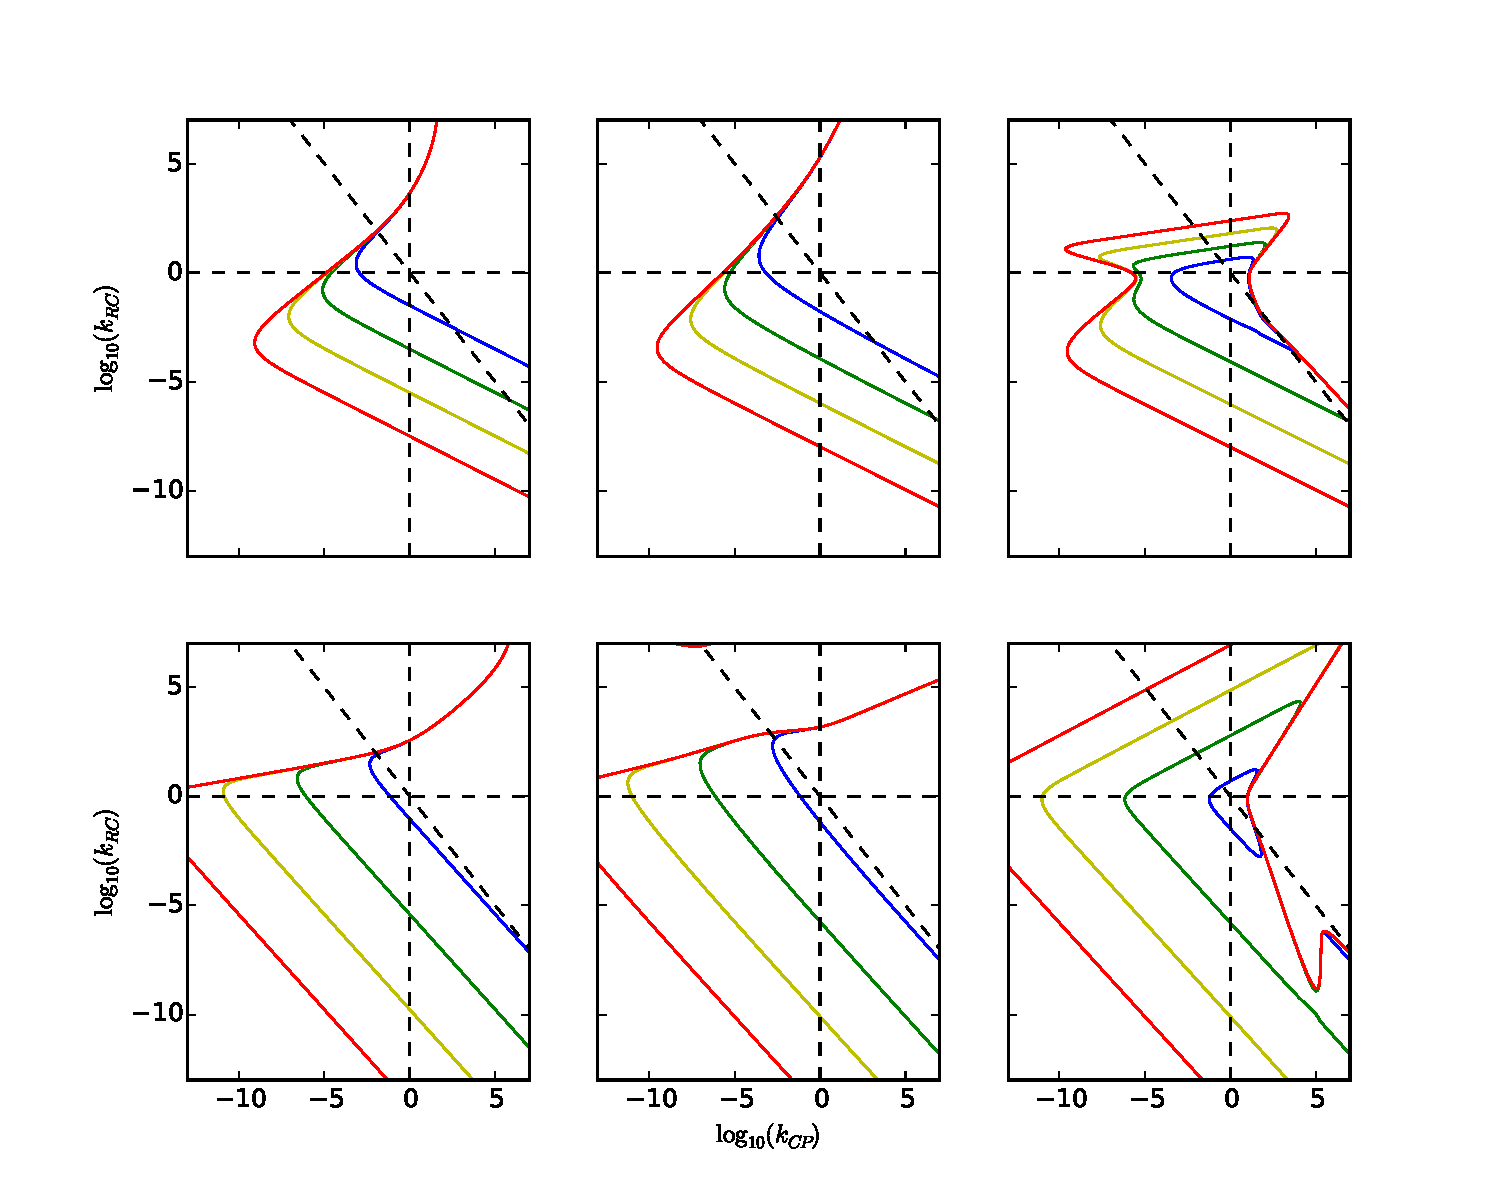
\includegraphics[width = 0.85\textwidth]{../manuscript/Plots/Z(IC4)AcGrGr.pdf}
\end{frame}

%---------------------------------------------------------------------------
\begin{frame}
  \frametitle{Invasibilidad $C \to P-R$}
  \begin{equation}
  c_\varepsilon = \frac{\varepsilon_2}{\varepsilon_1\varepsilon_3}
\end{equation}
\begin{columns}
  \begin{column}{0.7\textwidth}
    \begin{equation*}
      \begin{aligned}
        \mu_4 &:= (\gamma_2 = \chi_3 + c_\varepsilon \chi_4 - q_{0,2} < 0 \ \lor \\ &m_P^{h + 1 - 2\beta} < \zeta_4(k_{\RC},k_{\CP}) = \frac{c_\varepsilon \chi_4}{\chi_3 + c_\varepsilon \chi_4 - q_{0,2}} \zeta_2 )
      \end{aligned}
    \end{equation*}
  \end{column}
  \begin{column}{0.3\textwidth}
    \begin{center}
      \resizebox{0.3\textwidth}{!}{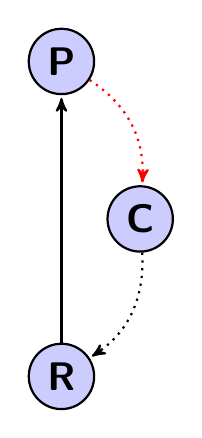
\begin{tikzpicture}[->,>=stealth',shorten >=1pt,auto,
  thick,main node/.style={circle,fill=blue!20,draw,font=\sffamily\Large\bfseries}]

\node[main node](R1) at (0,0) { R};
\node[main node](P1) at (0,4) {P};
\node[main node](C1) at (1,2){C};

\path
(R1) edge (P1)
(C1) edge[bend left,dotted] (R1)
(P1) edge[bend left,dotted,red] (C1);
\end{tikzpicture}
}
    \end{center}
  \end{column}
  \end{columns}

\end{frame}
% ---------------------------------------------------------------------------
\begin{frame}
  \frametitle{$C \to P-R$}
  \centering
  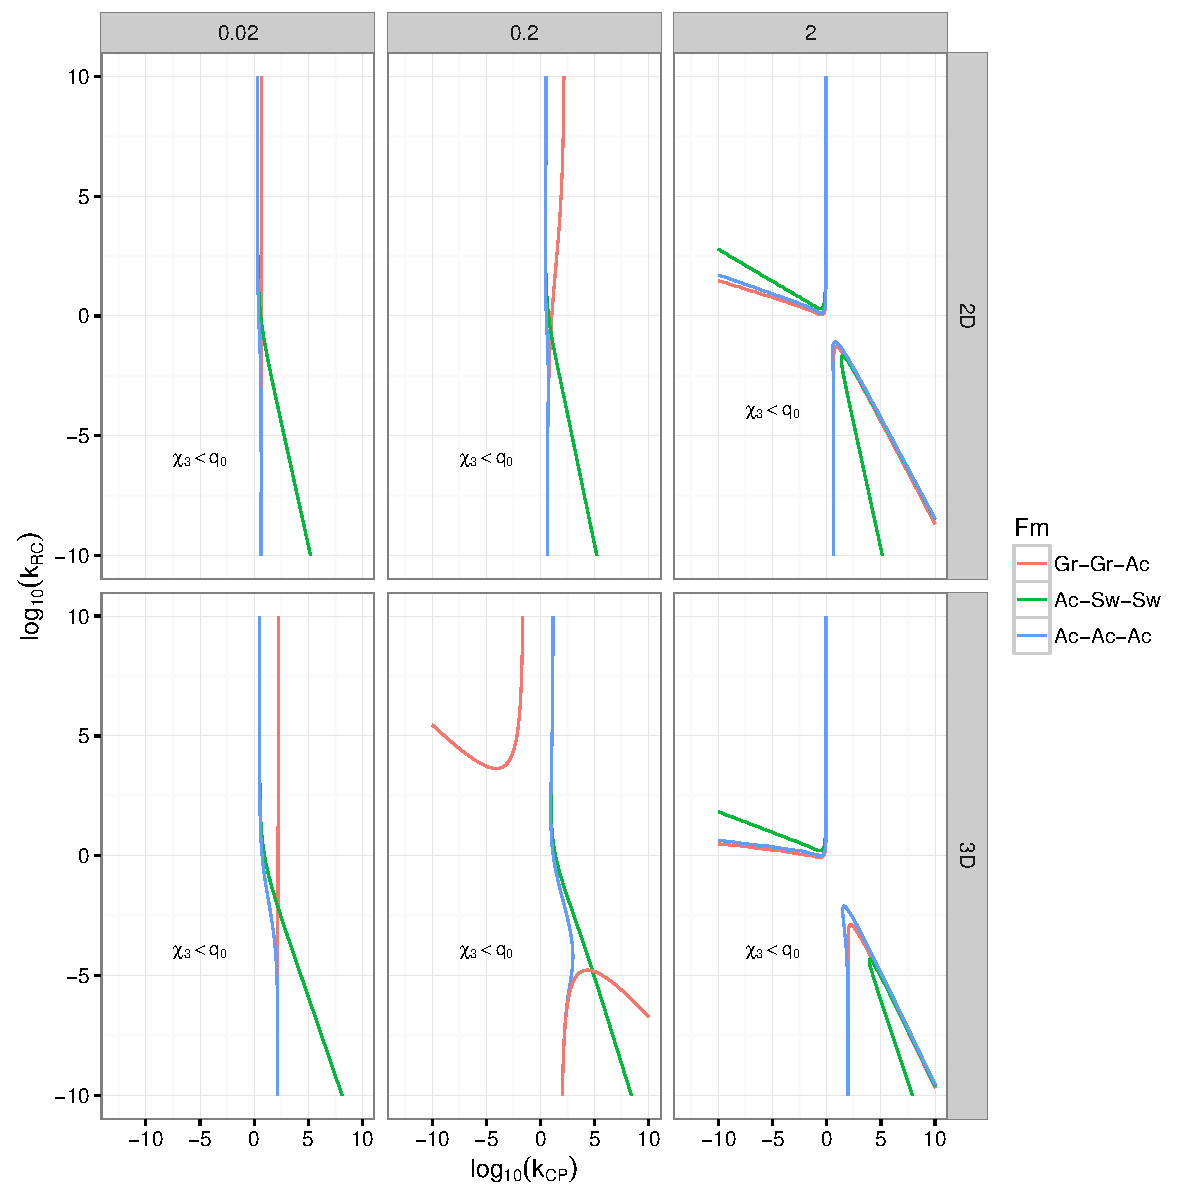
\includegraphics[width = 0.75\textwidth]{../manuscript/Plots/NecCPR.pdf}
\end{frame}
% ---------------------------------------------------------------------------
\begin{frame}
  \frametitle{$C \to P-R$}
  \begin{equation}
\mathbf{Z(I_{\CC \to \PP-\R})} := \{ (k_{\RC},k_{\CP},m_P) \in \mathbb{R}^3_+ / \mu_4 \land \mu_3 \}
\end{equation}

  \centering
  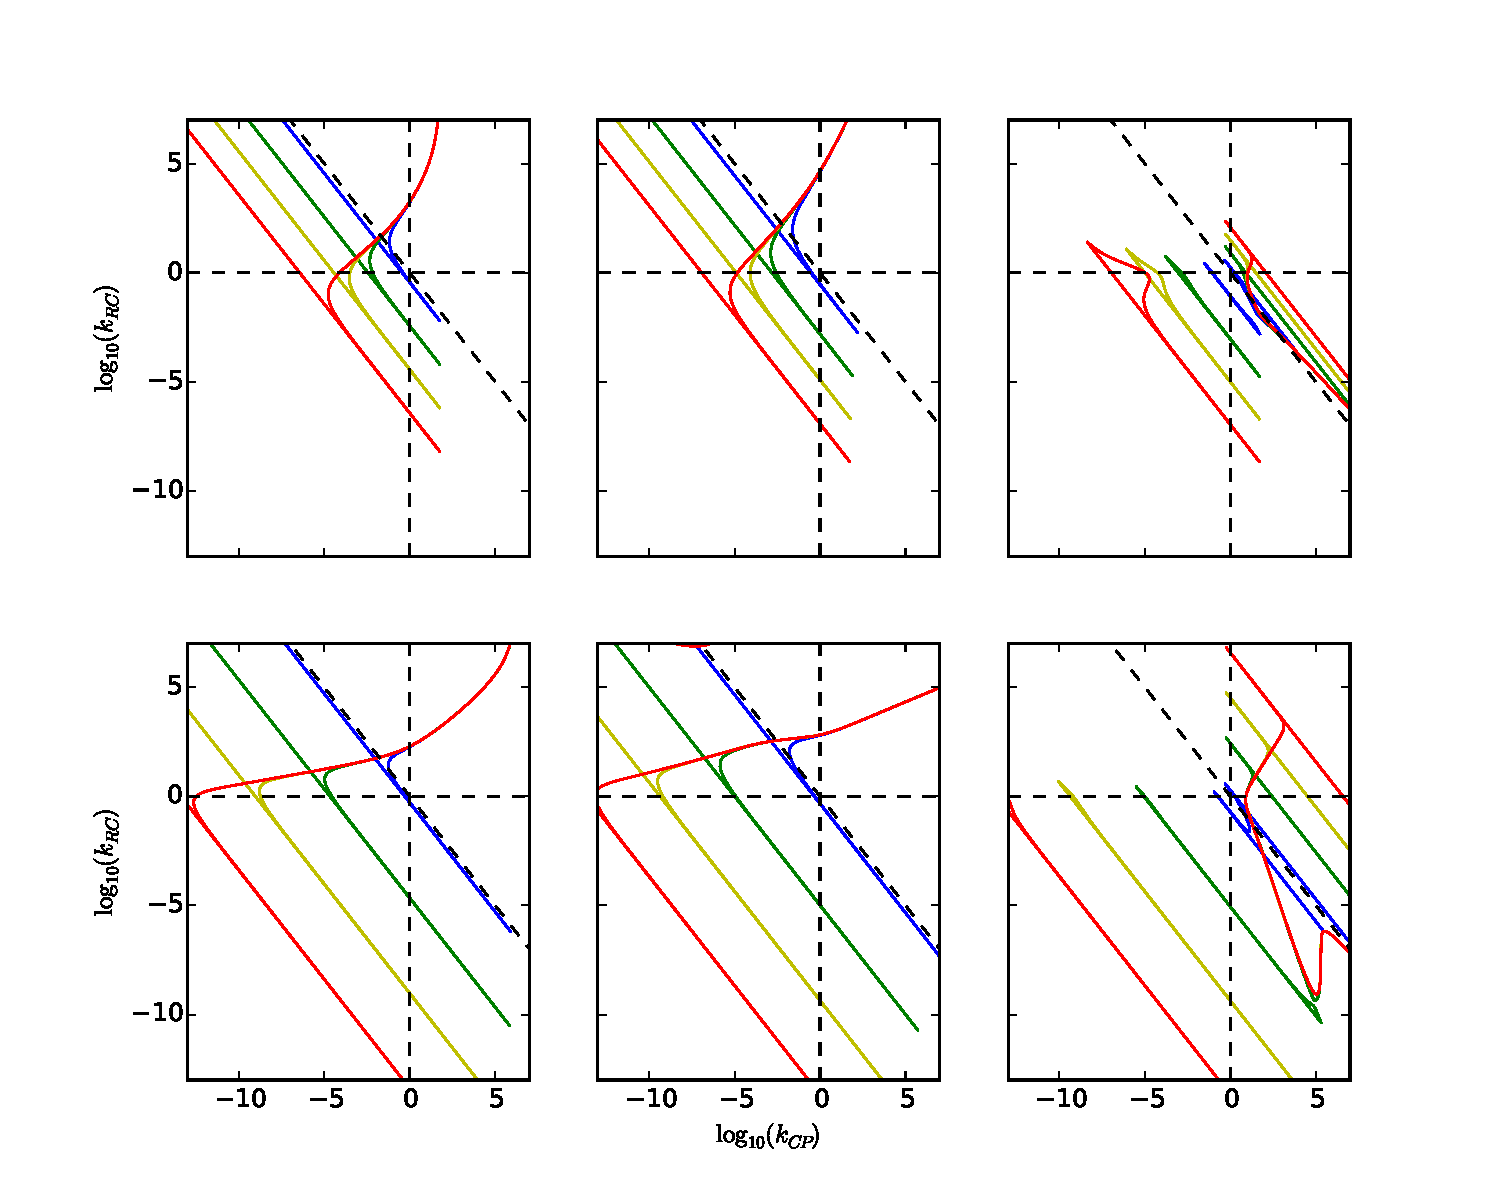
\includegraphics[width = 0.75\textwidth]{../manuscript/Plots/Z(IC5)AcGrGr.pdf}
\end{frame}
% --------------------------------------------------------------------------
\begin{frame}
  \frametitle{Invasibilidad Mutua}
  \begin{equation}
\mathbf{Z_{IM}} := \{ (k_{\RC},k_{\CP},m_P) \in \mathbb{R}^3_+ / \mu_1 \land \mu_2 \land \mu_3 \land \mu_4 \}
\end{equation}
\centering
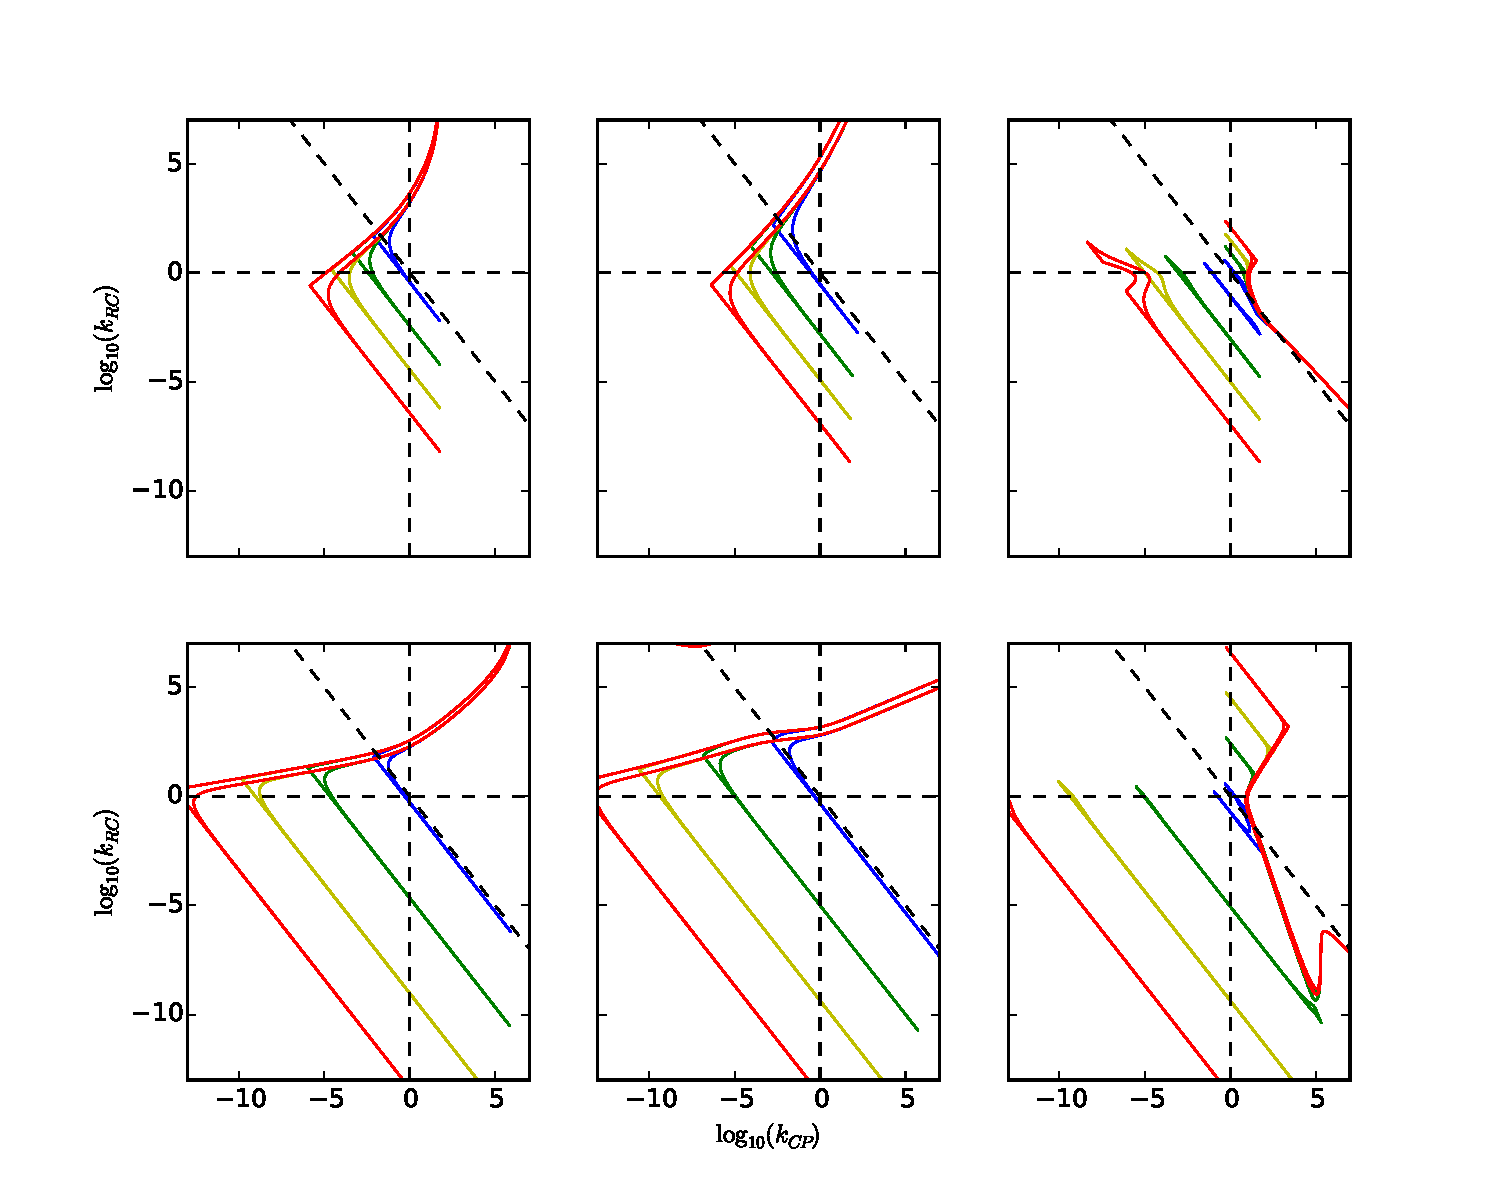
\includegraphics[width = 0.75\textwidth]{../manuscript/Plots/MutualInvAcGrGr.pdf}

\end{frame}
% ---------------------------------------------------------------------------
\begin{frame}
  \frametitle{Coexistencia}
  \begin{flalign*}
R^* &= \frac{K(\epsilon_3 ( \alpha_2 q_1 + \alpha_3 r) - \alpha_1 q_2)}{A}& \\
C^* &= \frac{K\alpha_1 \alpha_2 \epsilon_1 q_2 - K \alpha_2 \epsilon_2 ( \alpha_2 q_1 + \alpha_3 r) + \alpha_3 q_2 r} {\alpha_3 A} \\
P^* &= \frac{K \alpha_1 (\alpha_2 \epsilon_2 q_1 + \alpha_3 \epsilon_1 \epsilon_3 r) - (K \alpha_1^2 \epsilon_1 q_2 + \alpha_3 \epsilon_3  q_1 r)}{\alpha_3 A }
\end{flalign*}
Donde :
\begin{equation*}
  A = K \alpha_1 \alpha_2 \varepsilon_1 \varepsilon_3(1-c_\varepsilon) + \alpha_3\varepsilon_3 r
\end{equation*}

\end{frame}
%---------------------------------------------------------------------------
\begin{frame}
  \frametitle{Coexistencia}
$A >0$ :
\begin{equation*}
  \mu_3 \land \mu_4
\end{equation*}
$A <0$ :
\begin{equation*}
  \lnot \mu_3 \land \lnot \mu_4
\end{equation*}

\pause
Condici\'on Necesaria
\begin{equation*}
  (R^*_C < R^*_P) \equiv (q_{0,2} > \chi_3)
\end{equation*}
\pause
\end{frame}
% ---------------------------------------------------------------------------
\begin{frame}
  \frametitle{Coexistencia}
  \centering
  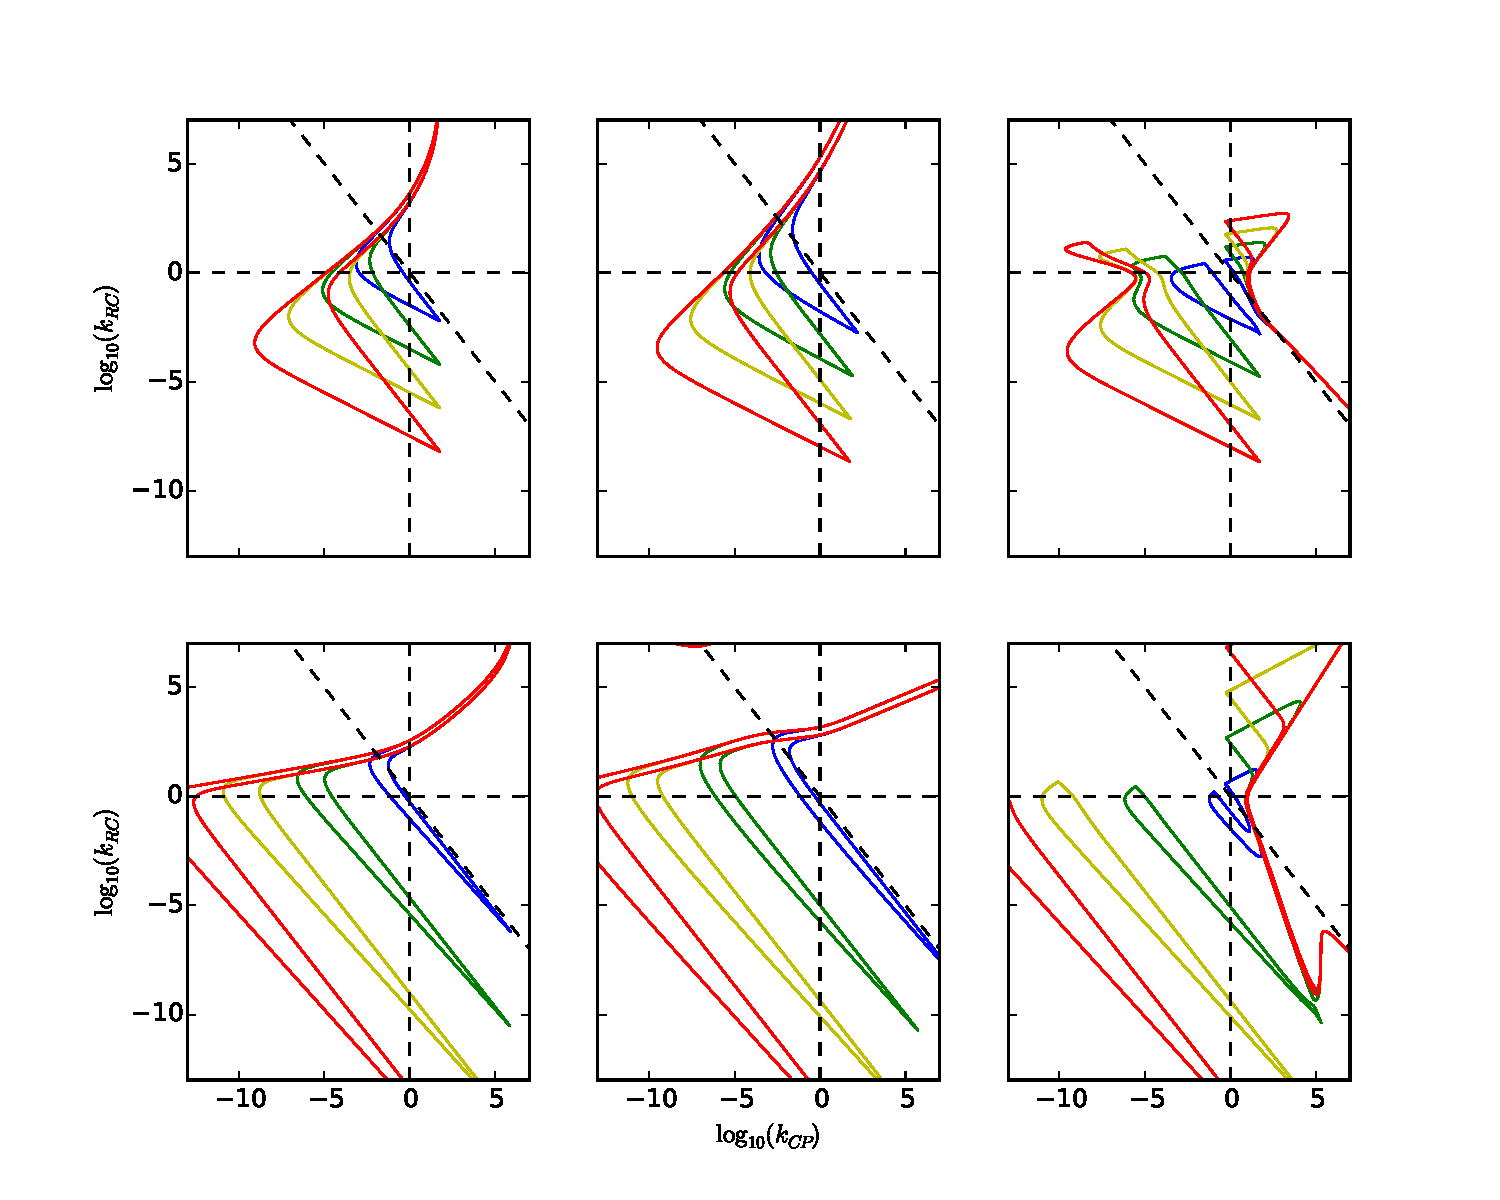
\includegraphics[width = 0.85\textwidth]{../manuscript/Plots/CoexistenceAcGrGr.pdf}
\end{frame}
% ---------------------------------------------------------------------------
\begin{frame}
  \frametitle{Estabilidad}
  \centering
  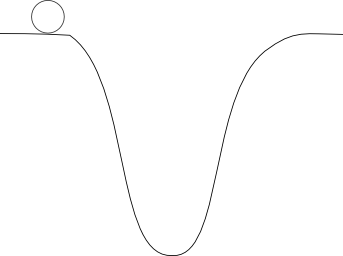
\includegraphics[width = 0.9\textwidth]{Pics/stability.png}
\end{frame}
% ---------------------------------------------------------------------------
\begin{frame}
  \frametitle{Estabilidad local}
  \begin{equation*}
    \frac{dx}{dt} = x \circ (r + A x)
  \end{equation*}
  \pause
  \begin{equation*}
    p(t) = det(M - tI) , \ M = Jac(\frac{dx}{dt})|_{x = x^*}
  \end{equation*}
  \pause
  \[p(\lambda) = 0 \]
  \pause
  \[\forall \lambda, \Re(\lambda) < 0 \]
    
\end{frame}

% ---------------------------------------------------------------------------
\begin{frame}
  \frametitle{Estabilidad local}
  Si $A < 0$ el equilibrio es localmente inestable
  \pause
  \begin{equation*}
    A > 0 \iff c_\varepsilon < 1 \  \lor \  m_P^{h + 1 - 2\beta} < \frac{c_\varepsilon \chi_4}{(c_\varepsilon - 1) \chi_2}
  \end{equation*}

  \begin{equation}
    \begin{aligned}
      \chi_2 &= \varepsilon_2 \kappa_0\alpha_{0,2} f_2(k_{\RP})k_{\RP}^{1-\beta} \\
      \chi_4 &= \frac{\varepsilon_3 \alpha_{0,3}r_0 f_3(k_{\CP})k_{\CP}^{\beta - h}}{\alpha_{0,1}f_1(k_{\RC})k_{\RC}^{1-\beta}}
    \end{aligned}
  \end{equation}
\end{frame}
% ---------------------------------------------------------------------------
\begin{frame}
  \frametitle{Estabilidad local} 
  \Large  Dado $A > 0$ tenemos que con la parametrizaci\'on usada:
  \begin{center}
    Coexistencia $\Rightarrow$ Estabilidad Local
  \end{center}
  \pause
  \begin{equation*}
    p(t) = t^3 + a_1t^2 + a_2t + a_3
  \end{equation*}
  \pause
  Criterio de \textit{Routh-Hurwtiz}
  \begin{equation}
    a_1 a_2 > a_3
  \end{equation}
  \pause
  Donde:
  \begin{equation}
    \begin{aligned}
      a_1 &= \frac{r}{K}R^* \\
      a_2 &= \alpha_2^2 \varepsilon_2 R^* P^*  + \alpha_1^2 \varepsilon_1 R^* N^*  + \alpha_3^2 \varepsilon_3 N^* P^*\\
      a_3 &= \frac{\alpha R^* N^* P^* A}{K} 
    \end{aligned}
  \end{equation}

\end{frame}
% ---------------------------------------------------------------------------
\begin{frame}
  \frametitle{Estabilidad local}
  \begin{equation}
    \begin{aligned}
      &B_0 [ \frac{\alpha_2}{\alpha_1}(m_P^{h - 2 \beta + 1} B_3 - B_4) + \frac{\alpha_1}{\alpha_2}(B_2 - B_1m_P^{h - 2 \beta + 1})] + \\ &\frac{K}{r} (m_P^{h-2 \beta + 1} B_3 - B_4) (m_p^{2 \beta - 1 - h} B_2 - B_1)  > 0
      \end{aligned}
\end{equation}

Donde:
\begin{equation}
  \begin{aligned}
    B_0 &= \alpha_{0,1}f_1(k_{\RC})k_{\CP}^{h - 1} ( \frac{\chi_3}{c_\varepsilon} + \chi_4 - q_{0,2})\\
    B_1 &= \frac{\varepsilon_1 \alpha_1 \alpha_{0,2} f_2(k_{\RP})}{\alpha_3}(\chi_3 + c_\varepsilon \chi_4 - q_{0,2}) \\
    B_2 &= \frac{r_0 q_{0,2} k_{\RP}^{2(\beta - 1)} }{\kappa_0} \\
    B_3 &= \frac{\alpha_1}{\alpha_3} \varepsilon_1 \alpha_{0,1} f_1(k_{\RC}) k_{\CP}^{h - 1}(\chi_3 + \chi_4 - q_{0,2})\\
    B_4 &= \frac{\varepsilon_3 q_{0,1} r_0 k_{\RP}^{2(\beta - 1)} k_{\CP}^{\beta - 1}}{\kappa_0}
  \end{aligned}
\end{equation}
\end{frame}
% ---------------------------------------------------------------------------

\begin{frame}
  \frametitle{Longitud de la cadena tr\'ofica}
  \begin{equation*}
    \begin{aligned}
      MTP &= 2 + \frac{\varepsilon_3 \alpha_3 C^*}{q_2} \\
      \frac{\varepsilon_3 \alpha_3 C^*}{q_2} &= \frac{K \alpha_1 \alpha_2 \varepsilon_3 \varepsilon_1 - K \alpha_2 \varepsilon_2 (\varepsilon_3/q_2) (\alpha_2 q_1 + \alpha_3 r) + \varepsilon_3 \alpha_3 r}{ K \alpha_1\alpha_2 \varepsilon_1 \varepsilon_3 - K \alpha_1\alpha_2 \varepsilon_2 + \varepsilon_3 \alpha_3 r}
    \end{aligned}
  \end{equation*}
  \pause
  Desviaciones de 3 se dan debido a:
  \begin{equation*}
      \frac{1}{c_\varepsilon} \chi_3 + \chi_4  > q_{0,2}
   \end{equation*}
\end{frame}
% -----------------------------------------------------------------------------
\begin{frame}
  \centering
  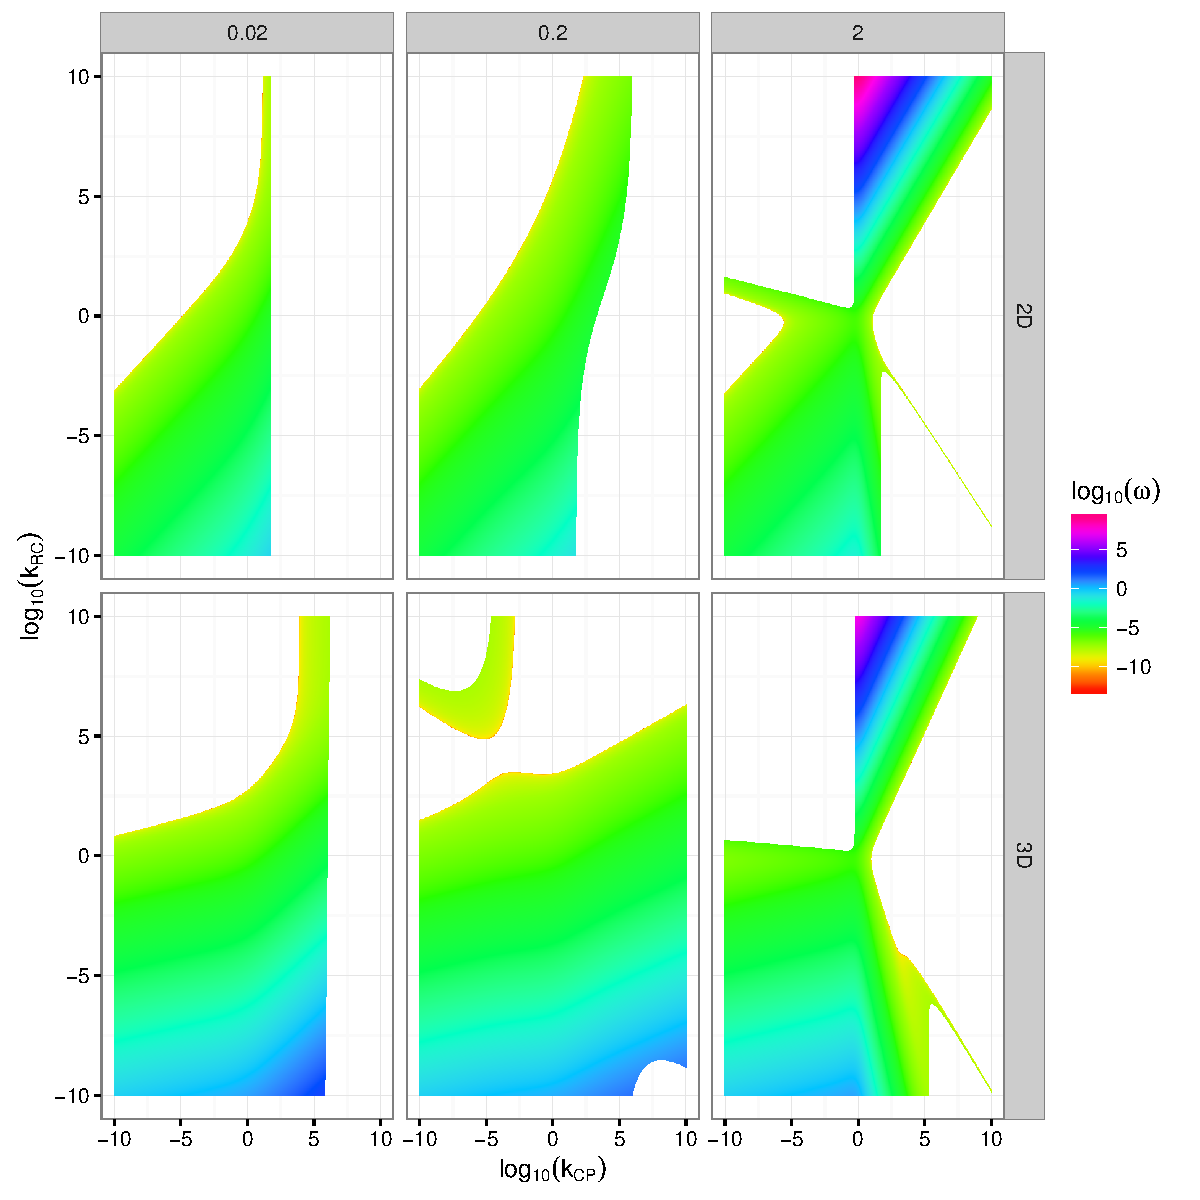
\includegraphics[width = 0.8\textwidth]{../manuscript/Plots/MTPvar.pdf}
\end{frame}
%-----------------------------------------------------------------------------
\begin{frame}
  \frametitle{An\'alisis de Datos}
  Red tr\'ofica de Benguela, \textit{Yodzis 1998}
  \centering
  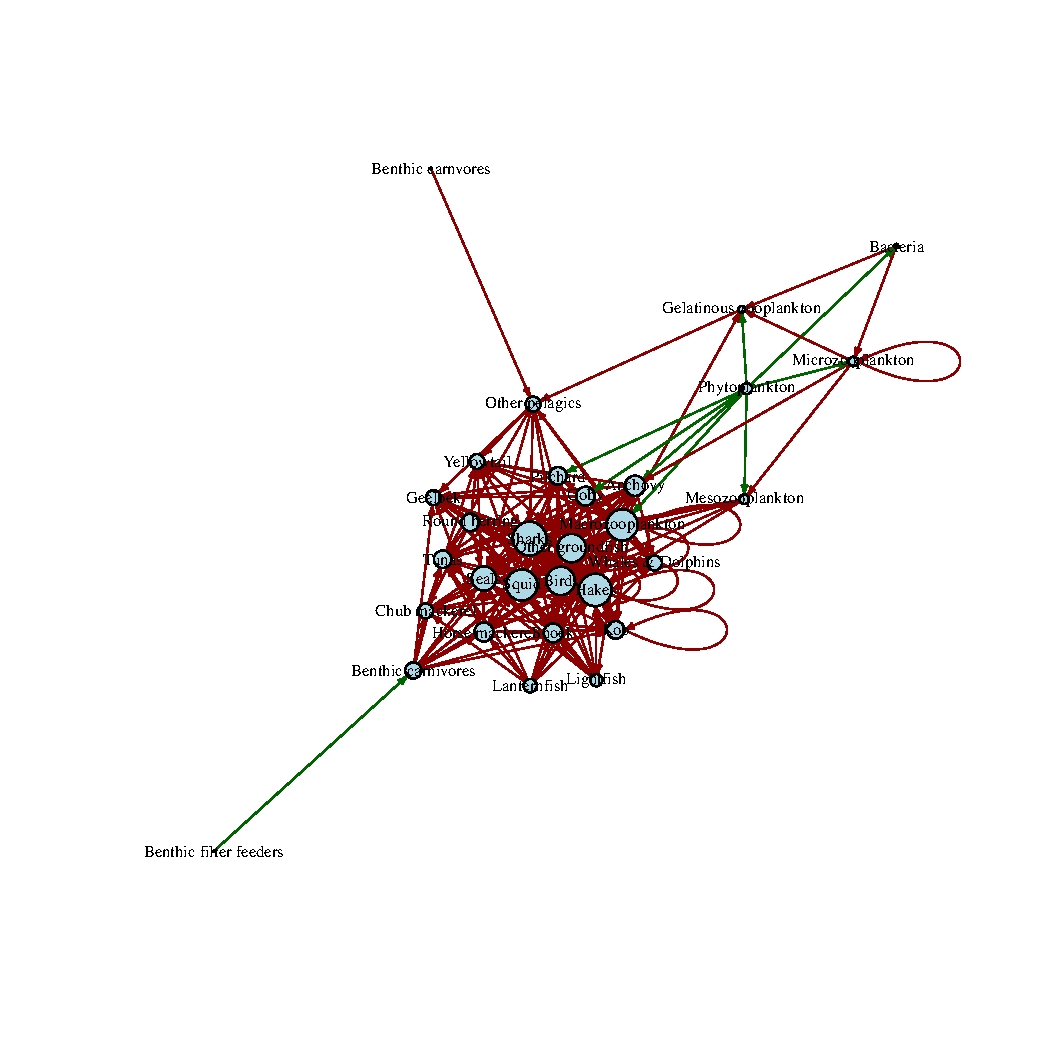
\includegraphics[width = 0.8\textwidth]{../manuscript/Plots/Benguela.pdf}
\end{frame}
%-----------------------------------------------------------------------------
\begin{frame}
  \frametitle{An\'alisis de Datos}
  \centering
  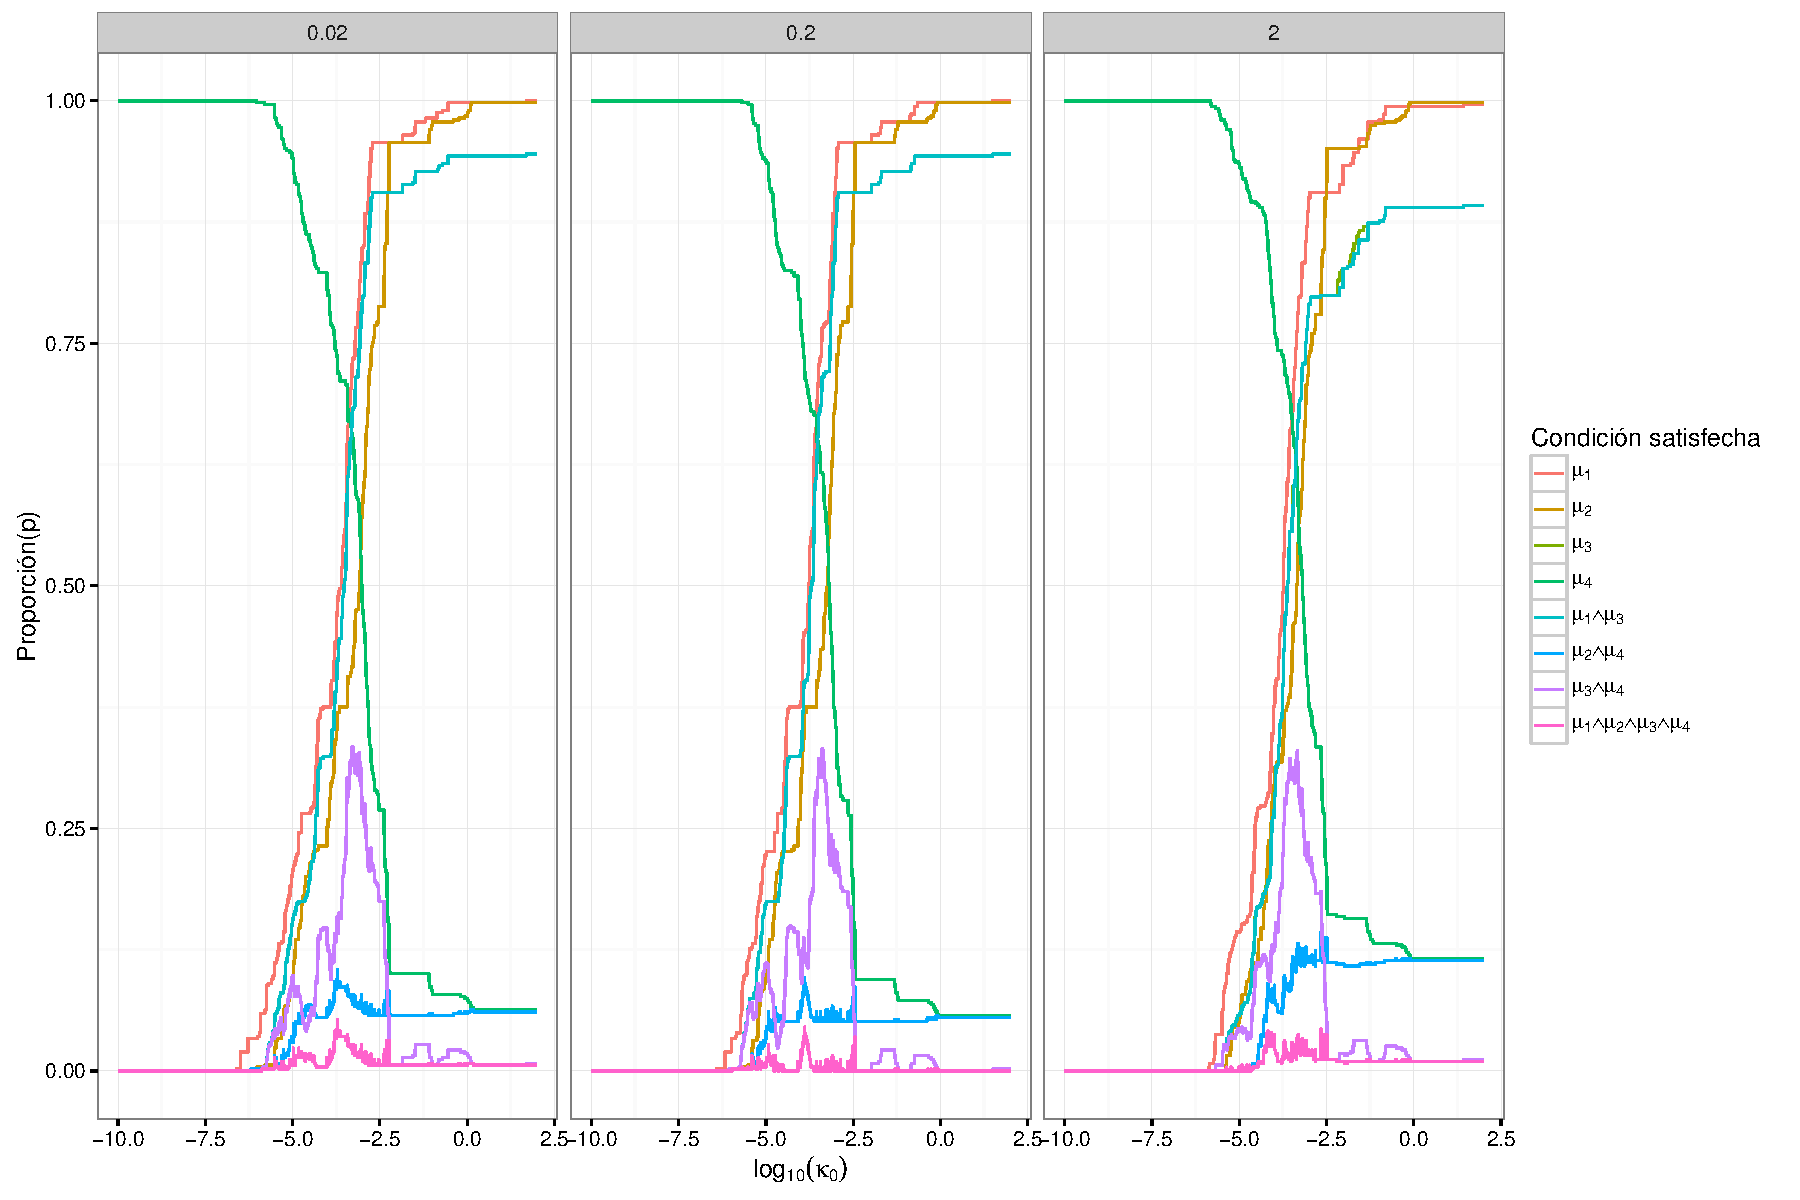
\includegraphics[width = \textwidth]{../manuscript/Plots/DataAna.pdf}
\end{frame}
%-----------------------------------------------------------------------------
\begin{frame}
  \frametitle{Conclusiones}
    \Large
  \begin{itemize}
  \item La distribuci\'on de masas presente en una comunidad modula la longitud de la cadena tr\'ofica
  \item La masa de las especies influencia los mecanismos de ensamblaje y coexistencia de las especies
  \item La forma de las relaciones ($\mu_i$) es independiente de la productividad del ambiente, la dimensi\'on del espacio de b\'usqueda y la combinaci\'on de estrategias de forrajeo
  \end{itemize}
\end{frame}
% ---------------------------------------------------------------------------
\begin{frame}
  \frametitle{Extensiones}
  \Large
  \begin{itemize}
  \item Inclusi\'on de los efectos de la temperatura
  \item Metacomunidades
  \item Efectos de la distribuci\'on de masas sobre el proceso de ensamblaje
  \end{itemize}
\end{frame}
% ---------------------------------------------------------------------------
\begin{frame}
  %\frametitle{Conclusions}
  \vspace{1 in}
  \begin{center}
    \Huge Gracias!
  \end{center}
\end{frame}
% ---------------------------------------------------------------------------
\begin{frame}
  \frametitle{Agradecimientos}
  \Large Walter Cabrera
  \centering
  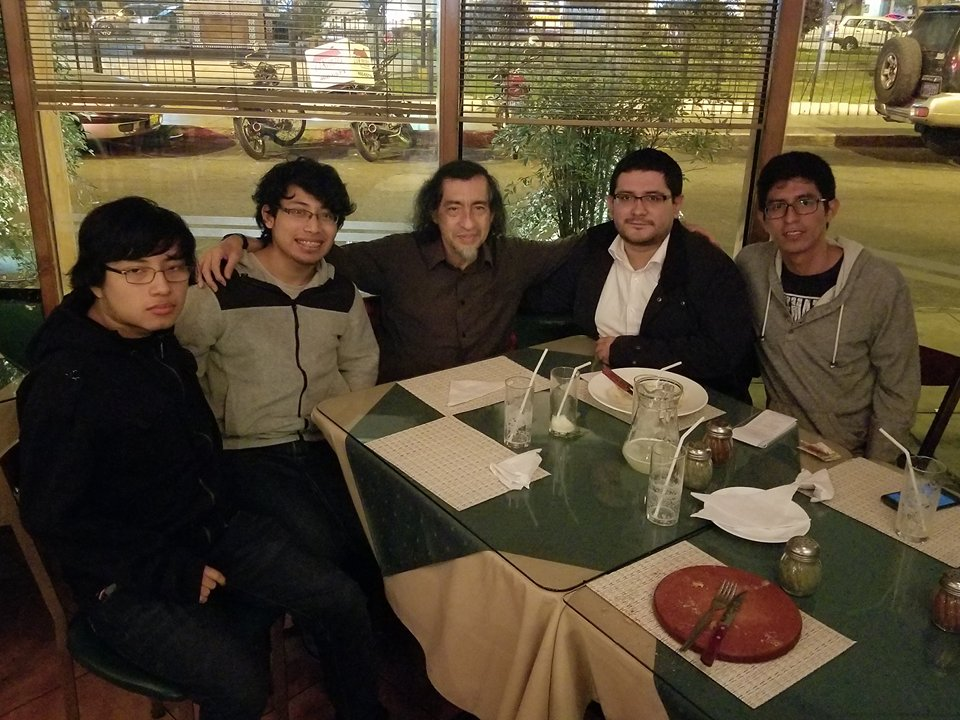
\includegraphics[width = 0.7\textwidth]{Pics/walter.jpg}
\end{frame}
% ---------------------------------------------------------------------------
\begin{frame}
  \frametitle{Agradecimientos}
  \Large Familia
  \centering
  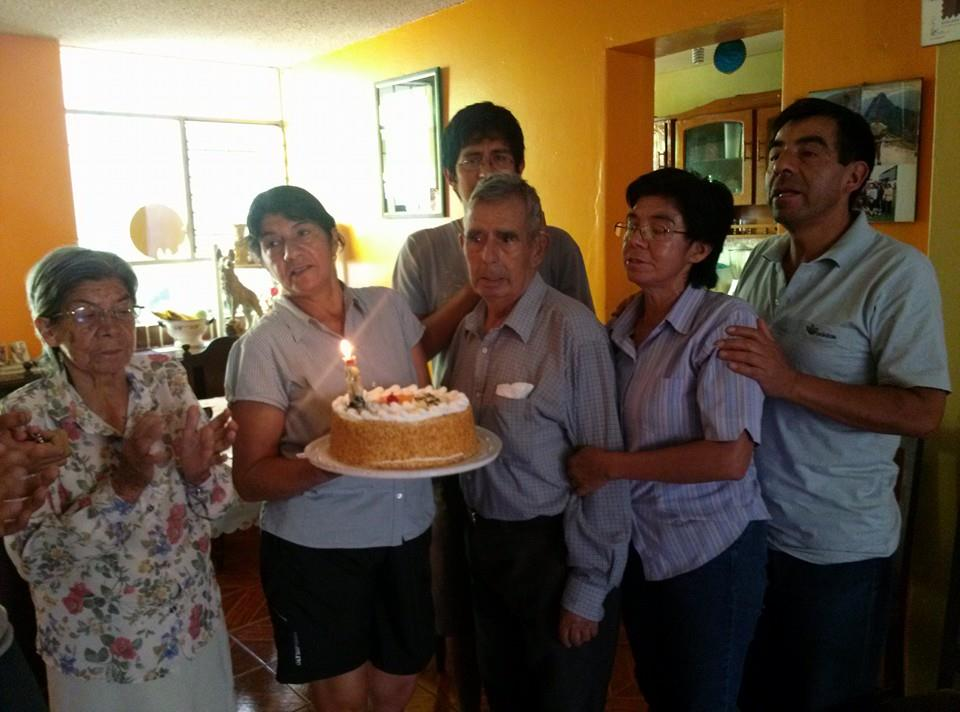
\includegraphics[width = 0.7\textwidth]{Pics/familia.jpg}
\end{frame}

\begin{frame}
  \frametitle{Agradecimientos}
  \begin{itemize}
  \item Lisveth Valenzuela
  \item Pedro Espinoza y Mart\'in Santiva\~nez
  \item Amigos de la Universidad
  \item Comunidad gamer: la T\'ia Jockey
  \end{itemize}
\end{frame}

\end{document}